%%%%%%%%%%%%%%%%%%%%%%%%%%%%%%%%%%%%%%%%%%%%%%%%%%%%%%%%%%%%%%%%
%% Vorlage fuer akademische Arbeiten, Gestaltungsrichtlinien der
%% Medienwissenschaft an der Universitaet Regensburg
%% 
%% Gutes Gelingen  --  Juli 2008
%% Christoph Mandl und Christoph Pfeiffer
%% http://www-mw.uni-r.de/studium/materialien 
%%
%% CC/BY-SA/3.0 - http://creativecommons.org/licenses/by-sa/3.0/
%%
%%%%%%%%%%%%%%%%%%%%%%%%%%%%%%%%%%%%%%%%%%%%%%%%%%%%%%%%%%%%%%%%
%%=============================================================%%
%%%%%%%%%%%%%%%%%%%%%%%%%%%%%%%%%%%%%%%%%%%%%%%%%%%%%%%%%%%%%%%%
%% Vorlage fuer akademische Arbeiten, Gestaltungsrichtlinien der
%% Medienwissenschaft an der Universitaet Regensburg
%% 
%% Gutes Gelingen  --  Juli 2008
%% Christoph Mandl und Christoph Pfeiffer
%% http://www-mw.uni-r.de/studium/materialien 
%%
%% CC/BY-SA/3.0 - http://creativecommons.org/licenses/by-sa/3.0/
%%
%%%%%%%%%%%%%%%%%%%%%%%%%%%%%%%%%%%%%%%%%%%%%%%%%%%%%%%%%%%%%%%%

%% koma script und ein paar optionen
\documentclass[%
%11.5pt%
12pt%
,oneside%
,a4paper%
%,normalheadings%
%,headsepline%
,liststotoc%
,bibtotoc%
,english%
,ngerman%
]{scrartcl}

\usepackage{xifthen}

%% soll automatisch nach Schriftverfuegbarkeit geprueft werden?
\newboolean{automatischeschriftwahl}
\setboolean{automatischeschriftwahl}{true}% true oder false

%% Inhaltsverzeichnisformate ansprechen
\usepackage[titles]{tocloft}

%% dvi - pdf - weiche
\ifx\pdftexversion\undefined
  \usepackage[dvips]{graphicx}
 \else
  \usepackage[pdftex]{graphicx}
 \fi

%% Satzspiegel
\usepackage[%
left=3.7cm%
,right=3.5cm%
,top=3cm%
,bottom=5cm%
,ignorehead%
]{geometry}

%% Zeilenabstand
\usepackage{setspace}
\setstretch{1.3}

%% Grundlegendes
\usepackage[latin1]{inputenc}
\usepackage[OT2, T1]{fontenc}
\usepackage[russian, german]{babel}
\usepackage{textcomp}


%%% >farbe< definieren
\usepackage[pdftex]{xcolor}
\definecolor{farbe}{gray}{0.30}
\definecolor{ueberschrift}{gray}{0.30}

%% einige wichtige pakete
\usepackage{%
ellipsis%
,fixltx2e%
,ae%
,verbatim%
,mparhack%
,xkeyval%
,enumitem%
,booktabs%
,lettrine%
,ragged2e%
,varioref%
}

%% Zitierzeichen damit kann schnell zwischen guillemets und anderen
%% gewechselt werden, ausserdem interessant f�r sprachspezifische
%% Zitierweisen. \foreignquote{language}{text}
%% Ersetzen der Texniccenter eigenen durch: "`-->\enquote{ und "'-->}
\usepackage[%
babel%
,german=guillemets%
]{csquotes}

\let\a\enquote

% dilletantische �nderung des Abstands �ber einer Section
\def\abstand{\quad\newline}

%% jurabib bibtex stilverwaltung
\usepackage{jurabib}
\usepackage{url,ifthen}
\jurabibsetup{commabeforerest,%
authorformat={year},titleformat=commasep,%
dotafter=bibentry,see,round,pages={format}}

%% weitere jurabib einstellungen
\renewcommand*{\bibbtsep}{In: }
\renewcommand*{\bibjtsep}{In: }
\renewcommand*{\biburlprefix}{[}%urls mit eckiger klammer
\renewcommand*{\biburlsuffix}{]}%urls mit eckiger klammer
%\renewcommand*{\biburlprefix}{\jblangle{}}% spitze-klammer-links
%\renewcommand*{\biburlsuffix}{\jbrangle{}}% spitze-klammer-rechts
\biburlfont{same} %Format:url
\AddTo{\bibsgerman}{%
\renewcommand{\Bibchaptername}{Kapitel}
\renewcommand{\editorname}{(Hrsg.)}}
\renewcommand*{\bibfnfont}{\textbf} %Format:Vorname
\renewcommand*{\biblnfont}{\textbf} %Format:Nachname
\renewcommand*{\bibtfont}{\textit} %Format:Titel
\renewcommand*{\bibbtfont}{\textit} %Format:Booktitle
\renewcommand*{\bibjtfont}{\textit} %Format:Journal
\renewcommand*{\bibapifont}{} %Format:Titel:unselbst�ndiger:Beitr�ge
\renewcommand*{\bibefnfont}{} %Format:Editor:Vorname
\renewcommand*{\bibelnfont}{} %Format:Editor:Nachname
\renewcommand{\bibaesep}{. } % Punkt nach Herausgebern
\renewcommand{\bibansep}{. } % Punkt nach (Jahr)
\renewcommand{\bibnumberformat}[1]{(#1)}
\renewcommand*{\jbcitationyearformat}[1]{(#1)} %Format:Jahreszahl
%% Autoren-Zwischenzeichen im Text
\renewcommand*{\jbbtasep}{ \& }
\renewcommand*{\jbbfsasep}{, }
\renewcommand*{\jbbstasep}{ \& }
%% Autoren-Zwischenzeichen  im LitVerz
\renewcommand*{\bibbtasep}{ {\textbf{\&}} }
\renewcommand*{\bibbfsasep}{{\textbf{;}} }
\renewcommand*{\bibbstasep}{ {\textbf{\&}} }
%% Herausgeber-Zwischenzeichen  im LitVerz
\renewcommand*{\bibbtesep}{ \& }
\renewcommand*{\bibbfsesep}{; }
\renewcommand*{\bibbstesep}{ \& }

%% Format fuer laengere Zitate
\newenvironment{zitat}{%
  \vspace{0.4cm}\begin{spacing}{1.1} \begin{addmargin}[1cm]{1cm} \list{}{%
  \small%
  }\item\relax}{\endlist \end{addmargin} \end{spacing}\vspace{3mm}}


%%% Seitenkopf und Seitenfu�
%\usepackage[automark]{scrpage2}
%	\pagestyle{scrheadings}
%	\setheadwidth[]{text}
%	\ihead{}
%	\chead{\headmark}
%	\ohead{}
%%	\setheadsepline{1pt}[\color{farbe}]
%\setheadsepline{1pt}
%	\cfoot{\pagemark}
%	\setkomafont{pagehead}{\itshape\small} 
%	\setkomafont{pagenumber}{\normalfont}
%
%%% eigener Seitenstil f�r Sections
%\defpagestyle{section}{%
%%{}{}{}}%
%(0pt,0pt){}{}{}(0pt,0pt)}%
%{{\pagemark\hfill}{\hfill\pagemark}{\hfill\pagemark\hfill}}
%
%%% eigener Seitenstil
%\defpagestyle{scrplain}{%
%{}{}{}}%
%{{\pagemark\hfill}{\hfill\pagemark}{\hfill\pagemark\hfill}}
%
%
%%% eigener Seitenstil
%\defpagestyle{nix}{%
%(0pt,0pt){}{}{}(0pt,0pt)}%
%{(0pt,0pt){}{}{}(0pt,0pt)}

%% Formate der Objektbeschriftungen
\addtokomafont{caption}{\itshape\small}
\setkomafont{captionlabel}{\itshape\bfseries\small}
\setkomafont{subparagraph}{\bfseries\small}

%% Fu�notenformatierung
\deffootnote[1.2em]{1.2em}{2.2em}{\thefootnotemark\ }

%% snake-oil f�r Bilder
\pdfcompresslevel=9 

% Hyperrefeinstellungen
\usepackage[%
unicode%
,a4paper%
,pdfpagelabels%
,pdftex%
]{hyperref}


%% Weitere Hyperrefeinstellungen
%% Fuer die jeweilige eigene Arbeit aendern!
\hypersetup{%
pdfauthor={Artur Spengler}%
,pdftitle={Syntax des Russischen: Eine Darstellung auf der Grundlage der Dependenzgrammatik}%
,pdfsubject={Syntax des Russischen: Eine Darstellung auf der Grundlage der Dependenzgrammatik}%
,pdfkeywords={Dependenzgrammatik, Grammatik, Russisch, Magister}%
,pdfcreator={\LaTeX with pdflatex and KOMA-Script}%
,pdfproducer={pdfetex}%
,pdfborder={0}%
,plainpages=false%
,breaklinks=true%
,pdfstartpage={1}%
,pdfpagelayout=OneColumn%
,pdfpagemode=UseOutlines%None,UseOutlines,UseThumbs,FullScreen 
%% fuer die Screen-Version: blue
%,linkcolor=blue,anchorcolor=blue,citecolor=blue,filecolor=blue,menucolor=blue,urlcolor=blue%
%% fuer die Print-Version: black
,linkcolor=black,anchorcolor=black,citecolor=black,filecolor=black,menucolor=black,urlcolor=black%
,colorlinks=true% Links farbig markieren oder mit Box umfassen 
,pdfhighlight=/I% 
,pdfborder=0 0 0%
}


%% Schein hat mehr Buchstaben als Sein.
%% Schriften:

% Mathe
\usepackage{amsmath}
\usepackage{amssymb}
\usepackage{amsthm}

\usepackage[scaled]{beramono} % Schreibmaschinenschrift: BeraMono

\ifthenelse{\boolean{automatischeschriftwahl}}{
%% wenn Adobe Stempel Garamond vorhanden ist, wird diese verwendet
\IfFileExists{t1pegj.fd}%
{%
\renewcommand{\rmdefault}{pegj}%
\usepackage[small,euler-digits]{eulervm}%
}{%
\usepackage{eco}%
\usepackage[osf]{mathpazo}%
}

%% wenn Adobe Myriad vorhanden ist, wird diese verwendet
\IfFileExists{t1fmy.fd}%
{%
\renewcommand{\sfdefault}{fmy}% Adobe Springer Myriad
}{%
%
}
}{}


%% freie Schriften
%\usepackage{eco}  %% medi�valziffern \oldstylenums \newstylenums
%\usepackage[osf]{mathpazo}  %% Palatino, plus passende Matheschrift

%% unfrei :
%%\usepackage[scaled,osf]{xagaramon}% Adobe Garamond Expert oldstylenums
%%\usepackage[scaled=1.03,osf]{xagaramon}% Adobe Garamond Expert oldstylenums, anders skaliert
%%
%\renewcommand{\rmdefault}{pegj}% Adobe Stempel Garamond oldstylenums
%\usepackage[small,euler-digits]{eulervm}
%%
%\renewcommand{\sfdefault}{fmy}% Adobe Springer Myriad
%%


%% snake-oil f�r den Satz
\pretolerance=100           %% Textsatz: interner Parameter zur Steuerung des Zeilenumbruchs
\tolerance 300              %% 1414 Bewertungsgrenzwert f�r schlecht umbrochene Zeilen
\hfuzz=0.2pt                %% Grenze, ab der eine overfull hbox gemeldet wird
\vfuzz=0.2pt                %% Grenzwert, ab dem die �berf�llung einer \vbox protokolliert wird
\hbadness 1414              %% Grenzwert f�r �schlechte� Zeilen, bzw. Boxen
\vbadness	1000              %% Grenzwert f�r eine �schlechte� \vbox 
\emergencystretch 1em       %% zus�tzlicher dynamischer Leerraum
\hyphenpenalty=30           %% Strafpunkte bei Silbentrennung �ber Absatz hinweg
\widowpenalty=100000          %% falls letzte Zeile auf neue Seite gebrochen wird.
\clubpenalty=100000           %% wenn erste Zeile eines Absatzes auf alter Seite bleibt.
\doublehyphendemerits=70    %% Aufeinanderfolgende Silbentrennungen eher vermeiden. 

%% microtype, optischer Randausgleich Extrusion und Protrusion
\usepackage[%
activate%
%,final%
%,verbose=true%
]{microtype}


% avoid page numbers being right-aligned in fixed-size box              
%\newlength{\newnumberwidth}
%\settowidth{\newnumberwidth}{99} % yields overfull hbox warnings for pages > 99
%\cftsetpnumwidth{\newnumberwidth}

%% Abstand im TOC vor sections
%\setlength{\cftbeforesecskip}{2em}%

%% sections
%\renewcommand{\cftsecpresnum}{\huge}% Nummerierung
%%\renewcommand{\cftsecnumwidth}{}% Breite der Nummernbox
%\renewcommand{\cftsecaftersnumb}{\hspace{0.3em}{\vspace{0.2em}}}% Nach Nummernbox, vor Titelbox
%\renewcommand{\cftsecfont}{\large\scshape}% Titelschrift
%\renewcommand{\cftsecleader}{\hspace{0.3em} $\cdot$ \hspace{-0.7em}}% Abstand und Zwischenzeichen
%\renewcommand{\cftsecpagefont}{\normalfont}% Seitenzahlschrift
%\renewcommand{\cftsecafterpnum}{\cftparfillskip}%
%\renewcommand{\cftsecindent}{0em}%
%{\relax}% 



%% subsections
%\renewcommand{\cftsubsecpresnum}{\textls}% Nummerierung
%\renewcommand{\cftsubsecnumwidth}{1.9em}% Breite der Nummernbox
%%\renewcommand{\cftsubsecaftersnumb}{\hspace{6em}}% Nach Nummernbox, vor Titelbox
%\renewcommand{\cftsubsecfont}{\normalfont}% Titelschrift
%\renewcommand{\cftsubsecleader}{\hspace{0.3em} $\cdot$ \hspace{-0.7em}}% Abstand und Zwischenzeichen
%%\renewcommand{\cftsubsecpagefont}{}% Seitenzahlschrift
%\renewcommand{\cftsubsecafterpnum}{\cftparfillskip}%
%\renewcommand{\cftsubsecindent}{0em}%
%{\relax}% 

%% subsubsections
%%\renewcommand{\cftsubsubsecpresnum}{}% Nummerierung
%\renewcommand{\cftsubsubsecfont}{\normalfont}% Titelschrift
%\renewcommand{\cftsubsubsecleader}{\hspace{0.3em} $\cdot$ \hspace{-0.7em}}% Abstand und Zwischenzeichen
%%\renewcommand{\cftsubsubsecpagefont}{}% Seitenzahlschrift
%\renewcommand{\cftsubsubsecafterpnum}{\cftparfillskip}%
%\renewcommand{\cftsubsubsecindent}{0em}%
%{\relax}%



%                
%    % figures     
%    	\renewcommand{\cftfigpresnum}{\scshape}% 
%    	\renewcommand{\cftfigfont}{\normalfont}%                 
%        \renewcommand{\cftfigleader}{\hspace{1.5em}} 
%        \renewcommand{\cftfigpresnum}{\figurename~}%Fig.~}
%        \renewcommand{\cftfigafterpnum}{\cftparfillskip}
%        \newlength{\figurelabelwidth}
%        \settowidth{\figurelabelwidth}{\cftfigpresnum~99}
%        \addtolength{\figurelabelwidth}{2.5em}
%        \cftsetindents{figure}{0em}{\figurelabelwidth}
%    % tables
%    	\renewcommand{\cfttabpresnum}{\scshape}%
%    	\renewcommand{\cfttabfont}{\normalfont}%
%        \renewcommand{\cfttableader}{\hspace{1.5em}} 
%        \renewcommand{\cfttabpresnum}{\tablename~}%Tab.~}
%        \renewcommand{\cfttabafterpnum}{\cftparfillskip}    
%        \newlength{\tablelabelwidth}
%        \settowidth{\tablelabelwidth}{\cfttabpresnum~99}
%        \addtolength{\tablelabelwidth}{2.5em}
%        %\cftsetindents{table}{0em}{\tablelabelwidth}
%        \cftsetindents{table}{0em}{\figurelabelwidth}


%% have the bib neatly positioned after the rest
%    \newlength{\beforebibskip}  
%    \setlength{\beforebibskip}{0em}   
       



%% Abk�rzung f�r \foreignlanguage{russian}{}

%\newcommand{\rus}{\foreignlanguage{russian}}
%\newcommand{\rus}{\fontfamily{ptm}\selectfont%
%                       \foreignlanguage{russian}}
                       
%\newcommand{\cyrbox}[1]{%
%  \mbox{\fontencoding{OT2}\fontfamily{wncyr}\selectfont#1}} 
%                       
\newcommand{\rus}[1]{%
  \mbox{\fontencoding{OT2}\fontfamily{wncyr}\selectfont#1}} 

\addto{\captionsngerman}{\renewcommand{\refname}{Quellenverzeichnis}}
\setkomafont{sectioning}{\rmfamily\bfseries\boldmath}
\setkomafont{caption}{\rmfamily\footnotesize\bfseries\boldmath}
\setkomafont{descriptionlabel}{\normalfont\bfseries}
\begin{document}
  %% Formatierungsdatei
%%=============================================================%%
\pagenumbering{roman}
%%================================= 
\begin{spacing}{1}
\begin{titlepage}

\begin{center}
\begin{LARGE}
\begin{scshape}
%Justus-Liebig-Universit�t Gie�en\\
\end{scshape}
\end{LARGE}

\vspace{1em}

\begin{figure}[h]
	\centering
		
\includegraphics{images/jlu-logo.pdf}
\end{figure}

\vspace{2em}

\begin{spacing}{1.5}
\begin{bfseries}
\Huge
\sffamily
Syntax des Russischen\\
\Large
Eine Darstellung auf der Grundlage der Dependenzgrammatik 

\end{bfseries}
\end{spacing}

\vspace{2em}

\normalsize
Magisterarbeit im Fach Slavische Sprachwissenschaft\\
Institut f�r Slavistik\\

\vspace{7em}


\begin{tabular}{rcl}
                              von: & \quad & Artur Spengler\\
                          Adresse: & \quad & Gr�nberger Stra�e 198\\
                                   & \quad & Zimmer 162\\[1em]
                                   & \quad & 35394~Gie�en\\[1em]
                   Matrikelnummer: & \quad & 601~096~3\\[1em]
                    Erstgutachter: & \quad & Prof.~Dr.~Monika~Wingender\\
                   Zweitgutachter: & \quad & Prof.~Dr.~Thomas~Daiber\\[1em]
               Laufendes Semester: & \quad & Wintersemester~2010/2011\\
                      Abgabedatum: & \quad & 28. Februar 2011\\
\end{tabular}
\end{center}
\end{titlepage}
\end{spacing}
%\newpage
%\cleardoublepage
%\phantomsection
%\thispagestyle{nix}
%\phantom{\LARGE{A}}

%%================================= 
%\pagestyle{scrheadings} %Kolumnentitel, siehe layout/format.tex
%%=================================
%%%%%%%%%%%%%%%%%%%%%%%%%%%%%%%%%%%%%%%%%%%%%%%%%%%%%%%%%%%%%%%%%
%% Vorlage fuer akademische Arbeiten, Gestaltungsrichtlinien der
%% Medienwissenschaft an der Universitaet Regensburg
%% 
%% Gutes Gelingen  --  Juli 2008
%% Christoph Mandl und Christoph Pfeiffer
%% http://www-mw.uni-r.de/studium/materialien 
%%
%% CC/BY-SA/3.0 - http://creativecommons.org/licenses/by-sa/3.0/
%%
%%%%%%%%%%%%%%%%%%%%%%%%%%%%%%%%%%%%%%%%%%%%%%%%%%%%%%%%%%%%%%%%

\cleardoublepage
\phantomsection

%\thispagestyle{section}
\abstand
\addcontentsline{toc}{section}{Vorwort}

\noindent \textbf{\textsf{\large }} \newline

\begin{spacing}{1.4}
\begin{figure}
\centering
\begin{minipage}{56mm}
\vspace{2cm}
\lettrine[lines=2, lhang=0.25, loversize=0.25, findent=3pt, nindent=0pt]{F}{�r} die Erstellung schriftlicher Arbeiten in der Regensburger Medienwissenschaft soll dieses kurze Dokument als Leitfaden dienen. Es behandelt sowohl allgemeine typografische Gesichtspunkte wie Lesbarkeit und �sthetik als auch formale Kriterien wie Aufbau der Arbeit und empfohlene Zitierweise. Die Richtlinien sind f�r Arbeiten in der Medienwissenschaft verbindlich und k�nnen sich im Einzelnen von Vorgaben in anderen F�chern unterscheiden.
\end{minipage}
\end{figure}
\end{spacing}
%%=================================
%%%%%%%%%%%%%%%%%%%%%%%%%%%%%%%%%%%%%%%%%%%%%%%%%%%%%%%%%%%%%%%%%%%
%% Vorlage fuer akademische Arbeiten, Gestaltungsrichtlinien der
%% Medienwissenschaft an der Universitaet Regensburg
%% 
%% Gutes Gelingen  --  Juli 2008
%% Christoph Mandl und Christoph Pfeiffer
%% http://www-mw.uni-r.de/studium/materialien 
%%
%% CC/BY-SA/3.0 - http://creativecommons.org/licenses/by-sa/3.0/
%%
%%%%%%%%%%%%%%%%%%%%%%%%%%%%%%%%%%%%%%%%%%%%%%%%%%%%%%%%%%%%%%%%

\cleardoublepage
\phantomsection
%\thispagestyle{section}
%\addcontentsline{toc}{section}{Zusammenfassung}
\abstand
\section{Zusammenfassung}

\vspace{1.2em}
\noindent Hier wird zusammengefasst. 
%%=================================
%%%%%%%%%%%%%%%%%%%%%%%%%%%%%%%%%%%%%%%%%%%%%%%%%%%%%%%%%%%%%%%%%%%
%% Vorlage fuer akademische Arbeiten, Gestaltungsrichtlinien der
%% Medienwissenschaft an der Universitaet Regensburg
%% 
%% Gutes Gelingen  --  Juli 2008
%% Christoph Mandl und Christoph Pfeiffer
%% http://www-mw.uni-r.de/studium/materialien 
%%
%% CC/BY-SA/3.0 - http://creativecommons.org/licenses/by-sa/3.0/
%%
%%%%%%%%%%%%%%%%%%%%%%%%%%%%%%%%%%%%%%%%%%%%%%%%%%%%%%%%%%%%%%%%

\cleardoublepage
\phantomsection
%\thispagestyle{section}
%\addcontentsline{toc}{section}{Abstract}
\abstand
\section{Abstract}

\vspace{1.2em}
\noindent This is for the abstract, hooray.
%%=================================
%%%%%%%%%%%%%%%%%%%%%%%%%%%%%%%%%%%%%%%%%%%%%%%%%%%%%%%%%%%%%%%%
%% Vorlage fuer akademische Arbeiten, Gestaltungsrichtlinien der
%% Medienwissenschaft an der Universitaet Regensburg
%% 
%% Gutes Gelingen  --  Juli 2008
%% Christoph Mandl und Christoph Pfeiffer
%% http://www-mw.uni-r.de/studium/materialien 
%%
%% CC/BY-SA/3.0 - http://creativecommons.org/licenses/by-sa/3.0/
%%
%%%%%%%%%%%%%%%%%%%%%%%%%%%%%%%%%%%%%%%%%%%%%%%%%%%%%%%%%%%%%%%%

\cleardoublepage
\phantomsection

\makeatletter
\renewcommand{\@dotsep}{10000}
\renewcommand{\@pnumwidth}{1.75em}
\renewcommand{\@tocrmarg}{2.75em}
\makeatother

\abstand
\setcounter{tocdepth}{2}
{\setstretch{1.3}{\tableofcontents}}
%%=================================
\pagenumbering{arabic}
%%=================================
%%%%%%%%%%%%%%%%%%%%%%%%%%%%%%%%%%%%%%%%%%%%%%%%%%%%%%%%%%%%%%%%
%% Vorlage fuer akademische Arbeiten, Gestaltungsrichtlinien der
%% Medienwissenschaft an der Universitaet Regensburg
%% 
%% Gutes Gelingen  --  Juli 2008
%% Christoph Mandl und Christoph Pfeiffer
%% http://www-mw.uni-r.de/studium/materialien 
%%
%% CC/BY-SA/3.0 - http://creativecommons.org/licenses/by-sa/3.0/
%%
%%%%%%%%%%%%%%%%%%%%%%%%%%%%%%%%%%%%%%%%%%%%%%%%%%%%%%%%%%%%%%%%

\cleardoublepage
\phantomsection

%\thispagestyle{section}
\abstand
\addcontentsline{toc}{section}{Einleitung}
\section*{Einleitung}

Die Syntax ist eine etablierte sprachwissenschaftliche Disziplin mit langer Tradition und hat dementsprechend eine F�lle von Modellen entwickelt, die sich teilweise erg�nzen, teilweise in unvereinbarer Konkurrenz zueinander stehen\footnote{\a{[...] es ist kaum zu bestreiten, dass es -- beim heutigen Stand unserer sprachwissenschaftlichen Erkenntnisse -- nicht nur vorkommt, dass zwei (oder mehr) Theorien dieselben fakten [sic] erkl�ren (und auch weitgehend ineinander �bersetzt werden k�nnen) oder dass eine Theorie prizipiell ad�quater ist als die andere, sondern dass oft auch zu beobachten ist, dass eine Theorie A die Sachverhalte a und b besser erkl�rt als eine Theorie B, die ihrerseits die Sachverhalte c und d besser zu erkl�ren vermag als die Theorie A} \citep[88]{Helbig1995}}. Zu den wichtigsten Vertretern der Syntaxforschung geh�ren zweifellos Noam Chomsky und Lucien Tesni�re.

Chomskys Konzept der Universalgrammatik als angeborenes kognitives Muster eines jeden Menschen bildet das Fundament f�r eine Reihe von Theorien und Untertheorien, die von zahlreichen Wissenschaftlern �ber die Zeit entwickelt und weitergef�hrt wurden. Dieses Theoriegeb�ude ist sehr abstrakt und wendet die Fragestellung von der Beschreibung der Struktur der �u�erung hin zur Beschreibung der �u�erungsproduktion und den zu Grunde liegenden Prozessen. Die �berschneidung zur Psychologie und Kognitionsforschung ist gro� und verleiht der Forschungsrichtung einen interdisziplin�ren Charakter. 

Tesni�res Dependenzgrammatik besch�ftigt sich mit der Struktur der �u�erung und gewann besonders in der p�dagogischen Anwendung eine nicht zu untersch�tzende Bedeutung. In kaum einem Einf�hrungswerk zur Linguistik fehlt ein Kapitel zur Dependenzgrammatik. �ber die Zeit entwickelte sich ein Geflecht von Formalismen, die auf dem Dependenz- und Valenzmodell beruhen, wie z.~B. die Tiefenkasustheorie oder die Kopfgesteuerte Phrasenstrukturgrammatik HPSG (Head Driven Phrase Structure Grammar).

Tesni�re z�hlte zu den ersten Mitgliedern des Prager Linguistenzirkels \citep[17]{Tesniere1980} und die sowjetische Akademiegrammatik \citep[13-82]{Svedova1980} stellt das Valenz- und Dependenzkonzept\footnote{Dort hei�t es jedoch \a{\rus{Podqinitelp1nye} \rus{svj1zi} \rus{slov} \rus{i} \rus{slovosoqetanij1}}; nach dem Begriff \rus{valentnostp1} sucht man vergebens, ebensowenig findet man Tesni�res Stemmata.} als Grundlage aller weiteren �berlegungen dar. Igor' Mel'\v{c}uks Arbeiten zum Text-Bedeutungsmodell \citep{Kahane2003} beinhalten Teile sowohl der Generativen Transformationsgrammatik als auch der Dependenzgrammatik.
In der russistischen Sprachwissenschaft als Ganzes betrachtet hat sich die Dependenzgrammatik aber nicht in der Form etablieren k�nnen so wie sie es etwa in der germanistischen Forschung getan hat.
\begin{zitat}
    Ein einheitlicher und methodisch wie theoretisch im Detail ausgearbeiteter Valenzbegriff ist [...] in der russistischen Sprachwissenschaft nicht in Sicht. \citep[1210]{Nuebler2003}
\end{zitat}
Dies verwundert.

Diese Arbeit stellt einen Versuch dar, zu er�rtern, wie gut sich die Dependenzgrammatik auf das Russische anwenden l�sst. Diese Frage erwuchs von einem computerlinguistischen Standpunkt, denn w�hrend meiner bisherigen Besch�ftigung mit kommerzieller Dependenz-Parsersoftware \citep{Spengler2008} stellte ich fest, dass gerade f�r das Russische Implementierungen fehlen. 
%Diese Beobachtung widerspricht der oben erw�hnten Durchdringung der Valenz- und Dependenzidee in den Grammatographien.
Die Frage nach der Anwendbarkeit ist unter anderem dadurch motiviert; sie d�rfte aber auch in anderen Kontexten interessant sein.

Die vorliegende Arbeit gliedert sich grob in zwei Teile, einen theoretischen und einen praktischen. Im ersten Teil f�hre ich in das Gebiet der Syntax ein und stelle neben anderen die Dependenzgrammatik vor, die ich auf knappem Raum mit der Konstituentenstrukturgrammatik und mit der Generativen Grammatik vergleiche. Bei den Ausf�hrungen zur Dependenzgrammatik st�tze ich mich im Wesentlichen auf Tesni�res Hauptwerk \citep{Tesniere1980}, erg�nzt durch neuere Arbeiten zum selben Thema; einen sehr breit gef�cherten Querschnitt des Forschungsstandes zu Dependenz und Valenz relevanten Themen bietet \citealp{Agel2003}.

Im praktischen Teil wende ich die Dependenzgrammatik auf konkrete russische S�tze an, die ich (mit Erlaubnis des Verlags) einem aktuellen Zeitungsartikel entnommen habe. Es handelt sich dabei um die Onlineausgabe der Zeitung \rus{Novaya Gazeta} \citep{Nikitinskiy2010}. Der Artikel ist im Anhang sowohl als Reintext als auch in einer dependenzgrammatisch annotierten Version zu finden. Ich hatte urspr�nglich vor, die Annotation listenartig zu gestalten, so dass in einer Zeile ein Wort st�nde, mit einer eindeutigen Nummer indexiert w�re und neben morphologischen Informationen einen Verweis auf die Indexnummer des Regens enthielte. Diese Variante h�tte nicht nur den Vorteil, gerademal halb so viel Platz in Anspruch zu nehmen, wie die graphische Darstellung, sondern auch maschinenverarbeitbar zu sein. Die Lesbarkeit f�r menschliche Betrachter litte indes sehr, und da ich diese Arbeit in erster Linie f�r menschliche Leser verfasst habe, entschied ich mich daf�r, die in der praktischen Untersuchung gefundenen Dependenzbeziehungen graphisch abzubilden.

Zuletzt noch ein Hinweis zu Quellenangaben und Fu�noten:\\
Literaturverweise habe ich stets im Flie�text direkt an der Stelle untergebracht, wo sich der Bezug zur Quelle befindet. Fu�noten habe ich verwendet, um zus�tzliche, f�r den Kern der Sache zwar entbehrliche, f�r das Verst�ndnis des Themas jedoch f�rderliche Informationen anzugeben. Es erscheint mir sinnvoll, derlei aus dem laufenden Text auszulagern, da es den Satz oder Absatz zu sehr aufbl�hen und die R�ckkehr aus dem Exkurs in den Lesefluss zu abrupt gestalten w�rde. Die Fu�noten k�nnen �bergangen werden, wenn der Leser es eilig hat.

%%=================================
%%%%%%%%%%%%%%%%%%%%%%%%%%%%%%%%%%%%%%%%%%%%%%%%%%%%%%%%%%%%%%%%
%% Vorlage fuer akademische Arbeiten, Gestaltungsrichtlinien der
%% Medienwissenschaft an der Universitaet Regensburg
%% 
%% Gutes Gelingen  --  Juli 2008
%% Christoph Mandl und Christoph Pfeiffer
%% http://www-mw.uni-r.de/studium/materialien 
%%
%% CC/BY-SA/3.0 - http://creativecommons.org/licenses/by-sa/3.0/
%%%%%%%%%%%%%%%%%%%%%%%%%%%%%%%%%%%%%%%%%%%%%%%%%%%%%%%%%%%%%%%%

\cleardoublepage
\abstand
\section{Syntax}
\label{sec:syntax:allgemein}

\subsection{Zum Begriff}
\label{subsec:begriff}

Syntax, (von griechisch 
$\sigma\acute{\upsilon}\nu\tau\alpha\xi\iota\varsigma$: Anordnung) ist neben der Morphologie eine Subdisziplin der Grammatik und bezeichnet einerseits den syntaktischen Bau der Sprache und andererseits die Lehre vom Satzbau, von der Ordnung, der die Satzglieder folgen und von den Satzgliedern selbst \citep[Vgl.][11]{Gabka1989}. Linke et al. heben weitere Bedeutungen des Begriffes hervor: Syntaktik bezeichnet in der Semiotik jegliche Relation zwischen Zeichen aller Art. So spricht man z. B. Von Wortsyntax, um die Beziehungen der Morpheme zu beschreiben, und von Textsyntax, um die Beziehungen der satz�bergreifenden textkonstituiernden Elemente zu beschreiben \citep[Vgl.][84]{Linke2004}. 

Der Begriff der Syntax findet auch au�erhalb der Untersuchung nat�rlicher Sprachen Verwendung, etwa in der Informatik, um die Struktur von Programmcode zu beschreiben. Ich beschr�nke mich allerdings auf die Bedeutung \a{Anordnung der nat�rlichsprachlichen W�rter zu nat�rlichsprachlichen S�tzen}.

Linke et al. \citep[85]{Linke2004} fassen die Regeln der Syntax f�r deutsche S�tze folgenderma�en zusammen:

\begin{zitat}
\begin{enumerate}
\item Damit eine Gruppe von W�rtern eine wohlgeformte Wortgruppe oder ein wohlgeformter Satz genannt werden kann, gen�gt es nicht, beliebige W�rter zusammenzustellen, sondern es braucht dazu ganz bestimmte W�rter, es braucht -- genauer gesagt -- syntaktische W�rter mit spezifischen Eigenschaften.
\item Es gen�gt auch nicht, die passenden W�rter mit den spezifischen Eigenschaften irgendwie zusammenzustellen; vielmehr muss eine bestimmte Ordnung eingehalten werden.
\item Damit etwas ein vollst�ndiger Satz ist, muss ein bestimmtes Minimum an W�rtern gegeben sein.
\end{enumerate}
\end{zitat}
Der Begriff \a{wohlgeformt} bedeutet so viel wie \a{akzeptabel, wenn auch nicht absolut grammatisch}. Obschon in der russischen Sprache auf Grund ihrer im Vergleich zum Deutschen m�chtigereren Morphologie die Wortstellung im Satz relativ frei ist, gelten die Regeln im Gro�en und Ganzen ebenso f�rs Russische.

Um S�tze bauen zu k�nnen, muss man sich also des Lexikons einer Sprache bedienen. Diese W�rter m�ssen mit Hilfe der Morphologie in eine gewisse Form gebracht werden. Und schlie�lich braucht es gewisser Regeln, mit denen diese morphologisch modifizierten W�rter miteinander in Beziehung gebracht werden.
Die Regeln des Satzbaus umfassen vom rein strukturalistischen Standpunkt lediglich das Vorhandensein von Satzteilen sowie ihre morphologische Beziehung zueinander -- die Morphologie ist von der Syntax nicht immer trennbar und die beiden Disziplinen werden zuweilen unter dem Begriff \a{Morphosyntax} zusammengefasst. Die sprachliche Richtigkeit allerdings erfordert dar�ber hinaus das Ber�cksichtigen semantischer Kriterien. So k�nnen nur solche W�rter miteinander kombiniert werden, deren semantische Eigenschaften wie z.B. Belebtheit, Beweglichkeit, Abstraktheit usw. miteinander kompatibel sind. Noam Chomskys vielzitiertes Beispiel f�r einen grammatisch korrekten, aber v�llig sinnlosen Satz \a{Colorless green ideas sleep furiously}, zu deutsch etwa \a{Farblose gr�ne Ideen schlafen zornig}, demonstriert dies deutlich.

Ein weiteres Kriterium, das im konkreten Kommunikationsprozess ber�cksichtigt werden muss, ist die Akzeptabilit�t. Grammatikalisch korrekte S�tze haben dann eine hohe Akzeptabilit�t, wenn sie vom H�rer problemlos verstanden werden. Die Akzeptabilit�t leidet z. B. dann, wenn die Satzl�nge oder die Anzahl der Satzglieder die Aufnahmef�higkeit des Kurzzeitged�chtnisses des H�rers �bersteigt \citep[Vgl.][149 f.]{Pelz2004}.

\subsection{Sinn der Disziplin}
\label{subsec:zweck}

Wie im vorherigen Unterkapitel festgestellt, liegt die Aufgabe der Syntax darin, die Regeln zu beschreiben, nach denen W�rter zu sinnvollen, akzeptablen und richtigen S�tzen kombiniert werden. Aber braucht man einen solchen Regelapparat �berhaupt? Wie sinnvoll ist es, sich Gedanken dar�ber zu machen, auf welche grundlegende Weise W�rter zu Satzverbunden gefasst werden? Betrachtet man die F�lle an konkurrierenden Grammatikmodellen, stellt sich zumindest die Frage, ob es eine einzige richtige Antwort �berhaupt geben kann. W�re es also nicht einfacher und naheliegender, alle m�glichen S�tze in einem S�tzebuch zu inventarisieren, so wie man W�rter in W�rterb�chern sammelt, und alle S�tze, die nicht im verbindlichen Verzeichnis gelistet sind, als ungrammatisch abzutun?

Man k�nnte es versuchen. Das S�tzebuch h�tte gewaltige Ausma�e und m�sste weit h�ufiger aktualisiert werden als jedes Lexikon. Wenngleich auch die Wortbildung Verfahren kennt, mit denen neue W�rter in die Sprache Eingang finden\footnote{Z.~B. Endung -itis an K�rperteilbezeichnung = entz�ndliche Krankheit}, ist die Menge der entstehenden Neologismen �berschaubar. Zudem h�lt sich die L�nge der entstehenden W�rter im Rahmen des lexikographisch verwertbaren -- abgesehen von Sprachen wie dem Deutschen, wo qua Komposition zumindest theoretisch unbegrenzt lange Wortneusch�pfungen entstehen k�nnen und im Papierdeutsch zuweilen beachtliche Bl�ten treiben\footnote{Z.~B. Bundesausbildungsf�rderungsgesetz, was jedoch dankbarerweise sofort wieder zu einem kryptischen Akronym eingedampft wurde: BAF�G.}. Mit dem Satzbau verh�lt es sich nun aber anders, denn die Anzahl der W�rter pro Satz ist theoretisch unbegrenzt und variiert in der Praxis stark, je nach stilistischer Richtung. M�ller f�hrt die beiden folgenden Beispiels�tze an, um zu demonstrieren, auf welche Weise ein Satz ins Unendliche in die L�nge gezogen werden k�nnte.

\begin{zitat}
    \begin{enumerate}
        \item Dieser Satz geht weiter und weiter und weiter und weiter . . .
        \item Ein Satz ist ein Satz ist ein Satz . . .
    \end{enumerate}
    \citep[1]{Mueller2008} 
\end{zitat}

Womit dieses Gedankenexperiment beendet und die Frage nach dem Sinn der Disziplin beantwortet ist: Die grundlegende Bauweise zu beschreiben ist die einzig sinnvolle Herangehensweise zur Untersuchung des Satzes.

Zur Mannigfaltigkeit der Syntaxtheorien bemerkt 

\subsection{Traditionelle Syntax}
\label{subsec:traditionelle:syntax}

Den Begriff \a{traditionell} klar zu definieren ist nicht einfach; Linke et al. \citep[59]{Linke2004} z�hlen alle Modelle, die in der Vergangenheit irgendwann vorgebracht wurden, dazu. Ich gehe in diesem Abschnitt jedoch lediglich auf die Beschreibung des Satzes ein, die man unter pr�skriptiver \a{Schulgrammatik} versteht, d.~h. so, wie man es von der Schule her kennt.

Die in der althergebrachten Syntax untersuchten Einheiten sind Wortf�gung\footnote{Den Terminus \textit{Wortf�gung}, im Russischen \rus{slovosoqetanie}, trifft man typischerweise in der russistischen Grammatik. In den abendl�ndisch orientierten Str�mungen ist der Begriff \textit{Phrase} gel�ufiger.} und Satz, wobei letzterer in einfachen und zusammengesetzten Satz unterschieden wird. Die Bestandteile der eben erw�hnten syntaktischen Einheiten sind W�rter, die n�chsth�here, durch S�tze konstituierte Einheit ist der Text. Pelz merkt an, dass es schwierig ist, festzumachen, was ein \a{Satz} �berhaupt ist und ob er etwa der langue oder der parole angeh�rt \citep[Vgl.][147\, ff.]{Pelz2004}. Nichtsdestotrotz mangelt es nicht an Definitionen des Begriffs Satz; als gemeinsames Merkmal kann man die in sich abgeschlossene semantische �u�erung betrachten. Bloomfield sagt es so:
\begin{zitat}
Der Satz ist eine unabh�ngige sprachliche Form, die durch keine syntaktische Beziehung in eine gr��ere sprachliche Form eingebettet ist.
\citep[148]{Pelz2004}
\end{zitat}
Dar�ber hinaus zeichnet sich ein Satz durch eine gewisse formale Struktur aus, die sich durch Morphologie und Intonation �u�ert. S�tze bestehen aus W�rtern, allerdings nicht aus den Lexemen, wie sie im W�rterbuch stehen, sondern aus den voll flektierten Wortformen, sozusagen aus syntaktischen W�rtern \citep[Vgl.][86]{Linke2004}. Die Morphologie f�gt der lexikalischen Bedeutung eine syntaktische hinzu, d.h. die einzelnen W�rter werden in eine Subjekt-Pr�dikat-Beziehung zueinander gesetzt. Die Intonation f�gt weitere Bedeutungen hinzu. Das wichtigste Merkmal des Satzes, die Pr�dikativit�t, wird aber auf all diesen Ebenen gemeinsam realisiert \citep[Vgl.][18\,f.]{Gabka1989}.

Modalit�t, das Verh�ltnis des Gesagten sowie die Einstellung des Sprechers zur Wirklichkeit, ist ein wesentliches Charakteristikum der Pr�dikativit�t. Ein weiteres Charakteristikum der Pr�dikativit�t ist die Temporalit�t, das zeitliche Verh�ltnis des Gesagten zum Redemoment. Durch die Intonation letztendlich wird nicht nur der Satztyp gekennzeichnet, sondern auch die Abgeschlossenheit des Satzes \citep[Vgl.][18\,f.]{Gabka1989}.


\subsection{Satzgliedlehre}
\label{subsec:satzgliedlehre}

Dass ein Satz nicht blo� aus W�rtern, sondern aus komplexeren Einheiten besteht, fand man im 19. Jh. heraus. Die Satzgliedrolle ist den W�rtern und Wortgruppen jedoch nicht inh�rent, sondern ergibt sich je nach Zusammenspiel mit anderen Einheiten. Um diese Einheiten zu klassifizieren und zu beschreiben entlehnte man die Begriffe Subjekt, Pr�dikat, Objekt usw. aus der Logiktheorie \citep[Vgl.][87]{Linke2004}.

Auch Pelz \citep[Vgl.][147]{Pelz2004} erw�hnt eine auf die aristotelesche Logik zur�ckzuf�hrende Satzdefinition, nach der \a{ein Satz sei, was Subjekt und Pr�dikat hat}. Als Subjekt wird das bezeichnet, wor�ber etwas ausgesagt wird, und als Pr�dikat wird das bezeichnet, was �ber das Subjekt ausgesagt wird.

Laut Belo\v{s}apkova \citep[697\,ff.]{Belosapkova1989} wird der Satz gebildet aus den hauptrangigen Satzgliedern Subjekt und Pr�dikat sowie den nebenrangigen Satzgliedern Objekt, adverbiale Bestimmung und Attribut. Satzglieder k�nnen koordiniert sein, wobei nur gleichartige Satzglieder in Frage kommen, wohingegen Subordination verschiedenartige Satzglieder erlaubt. Die Kombination aus blo�em Pr�dikat und blo�em Subjekt benennt Belo\v{s}apkova \textit{\rus{predikativnyi0 minimum}}, Gabka \citep[Vgl.][45\,ff.]{Gabka1989} spricht im selben Zusammenhang von \textit{Satzkonfiguration}. In den F�llen, in denen das Pr�dikat ein Objekt fordert, geh�rt auch dieses zur Satzkonfiguration.

D�rscheid \citep[34]{Durscheid2010} benennt die prototypischen Merkmale des Subjekts 
% im Deutschen\footnote{Die russische Grammatikschreibung ist damit und mit den folgenden Beschreibungen der anderen Satzglieder konform. \citep[Vgl.][]{Svedova1980}}
wie folgt:

\begin{zitat}
    \begin{itemize}
        \item Das Subjekt ist mit \a{wer oder was} erfragbar (semantisches Kriterium).
        \item Das Subjekt ist das, wor�ber man spricht (pragmatisches Kriterium).
        \item Das Subjekt ist kongruenzausl�send (formales Kriterium).
        \item Das Subjekt wird in der Regel durch eine NP im Nominativ realisiert (formales Kriterium).
        \item Das Subjekt f�llt weg im Infinitiv (syntaktisches Kriterium).
    \end{itemize}
\end{zitat}

D�rscheid (ebd.) merkt gleichwohl an, dass nicht jedes dieser Kriterien uneingeschr�nkt gilt, so lassen sich Beispiele (wenn auch grenzwertig akzeptable) finden, in denen das eine oder andere Kriterium scheinbar au�er Kraft gesetzt ist. Im Wesentlichen kann man die Kriterien als Daumenregel gut gebrauchen.

F�r das Pr�dikat listet D�rscheid \citep[35]{Durscheid2010} die folgenden Merkmale auf:

\begin{zitat}
    \begin{itemize}
        \item Das Pr�dikat ist das Satzglied, dem kategorial nur eine Wortart, ein Verb bzw. ein Verbkomplex, entspricht (formales Kriterium).
        \item Das Pr�dikat bezeichnet eine auf das Subjekt bezogene Handlung, einen Vorgang oder einen Zustand (semantisches Kriterium).
        \item Das Pr�dikat ist durch Kongruenz auf das Subjekt bezogen (morphologisches Kriterium).
    \end{itemize}
\end{zitat}

Das Objekt wird bei D�rscheid \citep[36]{Durscheid2010} nach direktem Objekt und indirektem Objekt unterschieden. F�r Aktivs�tze gilt: Das direkte Objekt ist diejenige Entit�t, die \a{von dem im Verb bezeichneten Geschehen direkt betroffen ist (Patiens)}, das indirekte Objekt ist diejenige Entit�t, \a{auf die das Geschehen nur mittelbar gerichtet ist (Rezipient)}.

\begin{zitat}
    \begin{itemize}
        \item Das Objekt ist Zielpunkt des verbalen Geschehens (pragmatisches Kriterium).
        \item Das Objekt tr�gt die semantische Rolle des Patiens bzw. des Rezipienten (semantisches Kriterium).
        \item Das Objekt ist im Kasus durch das Verb (z.~B. \textit{treffen} + Akkusativ) oder durch das Adjektiv gestimmt (z.~B. \textit{treu} + Dativ) (formales Kriterium).
    \end{itemize}
\end{zitat}

Der Vollst�ndigkeit des Begriffsfeldes halber will ich auch den Begriff \a{Agens} an dieser Stelle einf�hren. Dieses bezeichnet den Urheber einer Handlung und ist in der Regel durch das Subjekt realisiert.

Das Adverbial definiert D�rscheid \citep[38]{Durscheid2010} wie folgt:

\begin{zitat}
    \begin{itemize}
        \item Adverbiale Bestimmungen beziehen sich auf das Verb (z.~B. \a{Er singt laut}) oder auf den ganzen Satz (z.~B. \a{Wahrscheinlich kommt er heute nicht}) (syntaktisches Kriterium)
        \item Adverbiale dr�cken die n�heren Umst�nde des Geschehens aus: den Ort (Lokaladverbial), die Zeit (Temporaladverbial), die Art und Weise (Modaladverbial), den Grund (Kausaladverbial) u.~a. (semantisches Kriterium).
        \item Adverbiale k�nnen realisiert werden als Adverbien (z.~B. \a{Er weinte sehr}), als PPs (z.~B. \a{Das Buch liegt auf dem Tisch}), als NPs (z.~B. \a{Er tanzte die ganze Nacht}) und als Nebens�tze (z.~B. \a{Er tanzte, bis die Sonne aufging}) (formales Kriterium).
    \end{itemize}
\end{zitat}

Das Attribut ist zwar kein Satzglied, stellt jedoch einen wichtigen Teil des tradtionellen syntaktischen Vokabulars dar und sollte darum an dieser Stelle nicht fehlen. D�rscheid definiert das Attribut \citep[43]{Durscheid2010} wie folgt:

\begin{zitat}
    \begin{itemize}
        \item Das Attribut ist eine Beif�gung zum Substantiv oder zum Adjektiv. Es ist nicht selbst Satzglied, sondern Teil eines Satzglieds (syntaktisches Kriterium).
        \item Als Attribute k�nnen verschiedene syntaktische Kategorien fungieren: APs (\a{kleine Kinder}), PPs (\a{das Buch auf dem Tisch}), NPs (\a{die Freundin meiner Nachbarin}), abh�ngige S�tze (\a{der Mann, der im Lotto gewonnen hat}) (formales Kriterium).
        \item Vom Pr�dikat abgesehen kann jdes Satzglied durch ein Attribut erweitert werden (syntaktisches Kriterium).
    \end{itemize}
\end{zitat}




%TODO Thema und Rhema durch andere Quellen als Gabka belegen
\subsection{Thema und Rhema}
\label{subsec:thema:rhema}

Ein Satz l�sst sich unterteilen in eine Subjektgruppe und eine Pr�dikatgruppe; zu letzterer werden auch die nebenrangigen Glieder gez�hlt. Je nach dem, welche der beiden Gruppen das Thema und welche das Rhema darstellt, entscheidet sich die aktuelle Gliederung des Satzes. Das Thema steht als Bindeglied zum vorhergehenden Text normalerweise vorn, das Rhema steht als das Neue und Wichtige hinten \citep[147\,f.]{Pelz2004}. In dialogischer Rede verzichtet man oft auf das Thema, so dass strukturell unvollst�ndige S�tze, die nur aus dem Rhema bestehen, entstehen \citep[Vgl.][23\,f.]{Gabka1989}.

Intonation wird als Mittel zum Hervorheben des Rhemas eingesetzt. Im Schriftlichen jedoch ist allein die Wortstellung von Belang. Abweichungen vom Muster Thema-Rhema sind durch Inversion m�glich: Insbesondere Frages�tze zeichnen sich dadruch aus, dass das Rhema h�ufig in form eines Interrogativpronomens am Anfang steht \citep[Vgl.][24\,ff.]{Gabka1989}.

%Die semantisch-intonatorische Einheit ist das Syntagma. Ein Syntagma kann aus einem Wort, einer Wortf�gung oder einer pr�dikativen Einheit bestehen, Voraussetzung ist, es bildet eine zusammenh�ngende, relativ abgeschlossene semantische Einheit. Diese ist innerhalb des Satzes verschiebbar. F�r das russische Syntagma ist eine lineare Anordnung der Bestandteile typisch. Ein Syntagma ist rhythmisch-melodisch hervorgehoben. Die syntagmatische Gliederung h�ngt mit der aktuellen Gliederung eng zusammen \citep[Vgl.][27\,ff.]{Gabka1989}.

\subsection{Komplexe S�tze}
\label{subsec:komplexe:saetze}

Die historische Entwicklung des komplexen Satzes aus einer Reihe von einfachen S�tzen spiegelt die zunehmend komplexe Auseinandersetzung der Menschen mit der Welt wider. Diese urspr�ngliche, formal nicht verbundene Abfolge gedanklich zusammenh�ngender S�tze hei�t asyndetische Parataxe (\rus{asindeticheski\"i parataksis}). Wenn die an sich eigenst�ndigen einfachen S�tze durch Konjunktionen verbunden sind, spricht man von syndetischer Parataxe.

Aus der Parataxe entwickelte sich die Hypotaxe, das Satzgef�ge. Zun�chst mussten aber die dazu notwendigen Bindemittel entwickelt werden. Die �lteste Form des Nebensatzes ist der anaphorische Relativsatz. Das Bindemittel zwischen Haupt- und Nebensatz ist ein Relativpronomen oder Relativadverb. Diese nehmen die Rolle des Subjekts im Nebensatz ein. Die subordinierenden Konjunktionen verbinden blo�, w�hrend die Korrelative (\rus{sootnositelp1noe slovo}) auf den nachfolgenden Nebensatz verweisen, der die eigentliche Information enth�lt. Korrelative haben Satzgliedfunktion.

Komplexe S�tze ohne formale Bindemittel k�nnen nicht immer klar nach Hypotaxe oder Parataxe unterschieden werden, da es manchmal m�glich ist, sowohl koordinierende Konjunktionen als auch subordinierende Mittel einzusetzen. Der Kontext kann hilfreich sein \citep[Vgl.][XX\,ff.]{Gabka1989}.

Das Satzgef�ge unterteilt sich in Hauptsatz und Nebensatz, wobei die Bezeichungen Haupt- und Neben- sich nicht auf den Inhalt beziehen, denn der Nebensatz kann durchaus die eigentliche Satzinformation tragen. Die aktuelle Gliederung ist davon unber�hrt. Die Termini beziehen sich auf rein formale Aspekte; der Nebensatz ist dem Hauptsatz auf syntaktischer Ebene untergeordnet.

Tats�chlich haben viele Nebens�tze die Funktion eines Satzglieds, andere nicht. Bei letzteren handelt es sich um weiterf�hrende Nebens�tze, die eine zus�tzliche Erg�nzung darstellen \citep[Vgl.][149\,f.]{Gabka1989}.

Abschlie�end sei angemerkt, dass ein komplexer Satz, wie er in der heutigen russischen Sprache beobachtet wird, in semantischer Hinsicht keineswegs auf eine Verbindung eigenst�ndiger einfacher S�tze reduziert werden darf. Derweil ein Hauptsatz ohne seine Nebens�tze als abgeschlossene semantische Einheit durchgeht, gilt dies mitnichten f�r einen Nebensatz, wenn er von seinem Hauptsatz getrennt betrachtet wird; die Satzproposition ver�ndert sich aber in beiden F�llen zwangsl�ufig. Dies gilt ebenso f�r die Parataxe \citep[Vgl.][719\,f.]{Belosapkova1989}.

\subsection{Syntaktische Besonderheiten}
\label{subsec:syntaktische:besonderheiten}

�u�erungen und Gedanken einer fremden Person werden durch spezifische syntaktische Konstruktionen wiedergegeben. Eingeleitet wird die fremde Rede (\rus{chuzhaya rechp1}) durch Verben des Sagens. Man unterscheidet die fremde Rede in direkte und indirekte Rede (\rus{pryamaya rechp1} und \rus{kosvennaya rechp1}), eine Mischform ist die erlebte Rede (\rus{nesobstvenno-pryamaya rechp1}). Im Kommunikationsprozess ist direkte und indirekte Rede vorherrschend, in der Belletristik kommt auch die erlebte Rede als stilistisches Mittel vor.

Die direkte Rede eignet sich, um mittels Intonation und Wortwahl den eigentlichen Urheber der Rede zu charakterisieren. Vom syntaktischen Standpunkt betrachtet ist die direkte Rede ein Nebensatz, der konjunktionslos von der einleitenden, selten nachgestellten oder mit der direkten Rede durchmischten Autorenrede (\rus{avtorskaya rechp1}) abh�ngt. 
Auch die indirekte Rede kann vor, nach, inmitten der Autorenrede oder um sie herum stehen und bildet einen von der Autorenrede abh�ngigen Nebensatz. 
Die erlebte Rede steht normalerweise nach der Autorenrede und ist entweder syntaktisch als Objektsatz oder als eigenst�ndiger Satz realisiert \citep[Vgl.][187\,ff.]{Gabka1989}. 

\subsection{Weitergehende Theorien}
\label{subsec:weitergehende:theorien}

Mit dem amerikanischen Strukturalismus bildeten sich neue Syntaxtheorien wie z.~B. Konstituentenstrukturgrammatik oder die Dependenzgrammatik, die eine eigene Terminologie entwickelten und sich zunehmend vom Konzept der klassischen Satzgliedlehre l�sten \citep[Vgl.][87]{Linke2004}. Die Motivation zur Entwicklung alternativer Grammatikmodelle besteht unter anderem darin, dass die klassische Satzgliedlehre nicht sicher definieren kann, was ein Satzglied ist, denn die Kriterien zur Unterscheidung der Glieder sind uneinheitlich: W�hrend Objekte der Form nach bestimmt werden (Akkusativ-Endung, Dativ-Endung, usw.), werden Adverbiale semantisch subklassifiziert (Ort, Zeit, usw.) Im Satz
\begin{zitat}
Ich h�nge das Bild an die Wand
\end{zitat}
\noindent kann nicht einwandfrei entschieden werden, ob es sich bei \a{an die Wand} um ein Objekt oder eine Adverbialbestimmung handelt \citep[Vgl.][88]{Linke2004}. Im selben Ma�e unklar ist sogar die Bestimmung des Subjekts: Ist im Satz
\begin{zitat}
Dem Lehrer ist ein Fehler unterlaufen
\end{zitat}
\noindent \textit{dem Lehrer} oder \textit{ein Fehler} das Subjekt? Laut heute g�ngiger Praxis, das Subjekt nach formalen Gesichtspunkten zu bestimmen, m�sste es \textit{ein Fehler} sein, also diejenige Einheit, die im Nominativ steht. Laut urspr�nglicher logischer Definition des Begriffs \textit{Subjekt}, wonach das ein Subjekt ist, wor�ber etwas ausgesagt wird, m�sste es aber \textit{der Lehrer} sein \citep[Vgl.][32]{Durscheid2010}.



%*********************************************************************
% Dependenzgrammatik *************************************************
%*********************************************************************
\clearpage
\abstand
\section{Dependenzgrammatik}
\label{sec:depenzgrammatik}

%Die Dependenzgrammatik hat insbesondere auf Grund ihrer starken Formalisierbarkeit und daraus resultierenden Verarbeitbarkeit mit Hilfe elektronischer Maschinen enorm an Bedeutung gewonnen.
%Ein mit der Dependenzgrammatik verwandtes und von ihr nicht zu trennendes Konzept ist das der Verbvalenz.

Die Dependenzgrammatik wurde von Lucien Tesni�re w�hrend seiner Kriegsgefangenschaft im Ersten Weltkrieg entwickelt \citep[11]{Weber1997}, in den 30er Jahren des 20. Jahrhunderts war die Theorie im Wesentlichen so weit, dass Tesni�re sie h�tte ver�ffentlichen k�nnen \citep[32]{Agel2000}. Publiziert wurde sein Hauptwerk \textit{�l�ments de syntaxe structurale} jedoch postum 1959 von seiner Frau und seinen Sch�lern, Tesni�re starb 1954. Im Laufe der Zeit beeinflusste und bef�rderte Tesni�res Modell der Dependenz und Regenz in der Beschreibung des Satzbaus eine Reihe weiterer Theorien, wie z.~B. die Lexikalisch-Funktionale Grammatik oder die Head-Driven Phrase Structure Grammar.

Kerngegenstand der Dependenzgrammatik nach Tesni�re ist die innere Ordnung, der die W�rter in einem Satz folgen. Tesni�re spricht von der \textit{ordre structural}, die er der \textit{ordre lin�aire} gegen�ber stellt. Realisiert wird die Strukturordnung durch drei Relationstypen, n�mlich
\begin{itemize}
    \item Konnexion
    \item Junktion
    \item Translation
\end{itemize}
Die Konnexion ist die grundlegende Verbindung zwischen W�rtern. Erst die Konnexion macht aus den W�rtern ein gr��eres Gebilde, dessen Bedeutung mehr ist als die einzelnen Bedeutungen der W�rter. Deshalb betrachtet man bei der Beschreibung eines Satzes die Relation als eine Komponente neben den W�rtern \citep[Vgl.][21]{Weber1997}.

Allerdings taugt nicht jede Wortart zur Bildung von Konnexionen, sondern nur solche, die selbst semantisch \a{gef�llt} sind, also lexikalische Bedeutung tragen. Allgemein bezeichnet man die Satzelemente, die durch Autosemantika realisiert werden, als Knoten oder Nuclei (Sg. Nucleus), Konnexionen finden also zwischen Nuclei statt. Nuclei werden stets in einem hierarchischen System angeordnet: ein Nucleus ist immer einem anderen unter- oder �bergeordnet, bzw. er h�ngt von ihm ab oder ist abh�ngig von einem anderen Nucleus. Daher der Name Dependenzgrammatik.

\subsection{W�rter}
\label{subsec:woerter}

Tesni�re entwickelte eine eigene Terminologie f�r W�rter, die er in die zwei Gruppen \textbf{Vollw�rter} und \textbf{Leerw�rter} unterteilte. Vollw�rter sind W�rter, die eigene lexikalische Bedeutung tragen, Leerw�rter haben lediglich eine grammatische Funktion im Satz (z.~B. Artikel, Pr�positionen etc.):
\begin{zitat}
    Volle W�rter nennen wir die mit semantischer Funktion, also die, deren Ausdrucksform unmittelbar mit einer Vorstellung verbunden ist, die sie darzustellen bzw. hervorzurufen haben. [...] Leere W�rter nennen wir die ohne semantische Funktion. Sie sind blo�e grammatische Hilfsmittel, deren Aufgabe einzig darin besteht, die Kategorie der vollen W�rter anzugeben, zu pr�zisieren oder auch zu �ndern und die Beziehungen zwischen vollen W�rtern zu regeln. \citep[28]{Tesniere1980}
\end{zitat}
Vollw�rter werden unterteilt in die vier Klassen Verb, Substantiv, Adjektiv (Epitheton) und Adverb (siehe Tabelle \ref{tab:vollwoerter}).

\begin{table}
    \begin{center}
        \begin{tabular}{ l  l }
            Klasse & Beispiel\\
            \hline
            Verb & \rus{pos�itp1}\\
            Substantiv & \rus{k�pka}\\
            Adjektiv (Epitheton) & \rus{st�ryi0}\\
            Adverb & \rus{nebr�z1nyi0}
        \end{tabular}
    \caption{Vollw�rter}
    \label{tab:vollwoerter}
    \end{center}
\end{table}

Leerw�rter unterteilt man in die beiden Klassen Junktoren und Translatoren (siehe Tabelle \ref{tab:leerwoerter}).

\begin{table}
    \begin{center}
        \begin{tabular}{ l  l }
            Klasse & Beispiel\\
            \hline
            Junktor & \rus{i}\\
            Translator & \rus{chto}\\
        \end{tabular}
        \caption{Leerw�rter}
        \label{tab:leerwoerter}
    \end{center}
\end{table}

Gesondert zu erw�hnen sind die Indizes, die als Indikatoren f�r grammatische Funktion dienen (z.~B. Artikel). Auch Anaphernw�rter nehmen eine Sonderstellung ein, da sie einerseits lexikalisch Leerw�rter sind, im Satz aber Vollw�rtern gleich Nuclei darstellen (siehe Abbildung \ref{fig:woerter} \citep[25]{Weber1997}).

\begin{figure}
    \begin{center}
        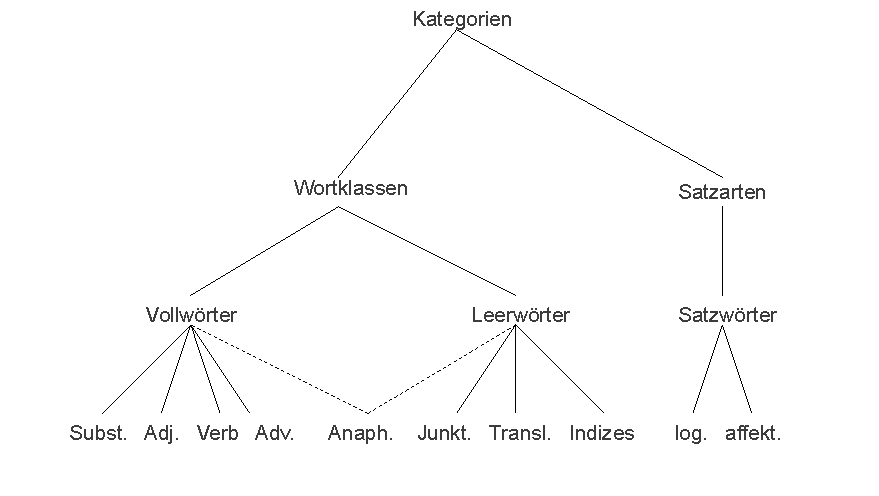
\includegraphics{images/woerter}
        \caption{W�rter}
        \label{fig:woerter}
    \end{center}
\end{figure}

Satzw�rter werden zwar als von den eigentlichen Wortklassen gesonderte Kategorie dargestellt, k�nnen jedoch prinzipiell durch jedes Vollwort realisiert werden. Typischerweise erscheinen in der Funktion des Satzwortes W�rter, die sich schwerlich als Autosemantika einstufen lassen. Es sind die logischen und affektiven Satzw�rter (siehe Tabelle \ref{tab:satzwoerter}).

\begin{table}
    \begin{center}
        \begin{tabular}{ l  l }
            Klasse & Beispiel\\
            \hline
            Logisches Satzwort & \rus{net}\\
            Affektives Satzwort & \rus{ah!}\\
        \end{tabular}
        \caption{Satzw�rter}
        \label{tab:satzwoerter}
    \end{center}
\end{table}

\subsection{Stemma}
\label{subsec:stemma}

Das Stemma (Pl. Stemmata) ist ein Diagramm zur Darstellung der Dependenzstruktur eines Satzes. Es besteht aus Kanten: Nichthorizontalen Linien, die das jeweilige Regens (Pl. Regentien) mit seinem Dependens (Pl. Dependentien) verbinden, wobei das Regens �ber dem Dependens positioniert ist. Die W�rter selbst konstituieren die Knoten, die durch Kanten verbunden werden. Um Regelm��igkeiten der Dependenz in einer Sprache oder auch sprach�bergreifend darstellen zu k�nnen, entwickelte Tesni�re Symbole f�r Knoten bzw. Vollwort-Klassen:\\
\\
I f�r Verb\\
O f�r Substantiv\\
A f�r Adjektiv\\
E f�r Adverb\\

Au�er den W�rtern aus diesen vier Klassen gibt es keine anderen, die Knoten bilden k�nnten. Das bedeutet, dass z.~B. Artikel zusammen mit dem Substantiv, das sie n�her bestimmen, in einen Knoten geschrieben werden und nicht etwa als Dependens unterhalb des Substantivs positioniert w�rden\footnote{Weber macht dies jedoch durchgehend. Er beruft sich fragw�rdigerweise darauf, dass Indizes manchmal -- etwa im Falle der den Substantiven �quivalenten Pronomina -- als Vollwortklasse behandelt werden \citep[Vgl.][42]{Weber1997}.}.

Die folgenden zwei Wortklassen bilden zwar keine Knoten, werden aber aufgrund ihrer Strukturrelevanz im Stemma explizit notiert:\\
\\
j f�r Junktor (siehe Kapitel \ref{subsec:junktion})\\
t f�r Translator (siehe Kapitel \ref{subsec:translation})\\
\\
Grunds�tzlich gelten Dependenzbeziehungen, wie in Tabelle \ref{tab:dependenzbeziehungen} dargestellt.

\begin{table}[htbp]
    \begin{center}
        \begin{tabular}{ c | l }
            Regens & m�gliches direktes Dependens\\
            \hline
            I & O, E\\
            O & A\\
            A & E\\
            E & E\\
        \end{tabular}
        \caption{Dependezbeziehungen zwischen Wortarten}
        \label{tab:dependenzbeziehungen}
    \end{center}
\end{table}

�gel \citep[37\,f.]{Agel2000} demonstriert dies anhand des Satzes \textit{Sehr sch�ne Frauen vergessen extrem h�ssliche M�nner �u�erst schnell}, das ein Stemma ergibt, wie in Abbildung \ref{fig:dependenzbeziehungen:beispielsatz} dargestellt.

\begin{figure}
    \begin{center}
        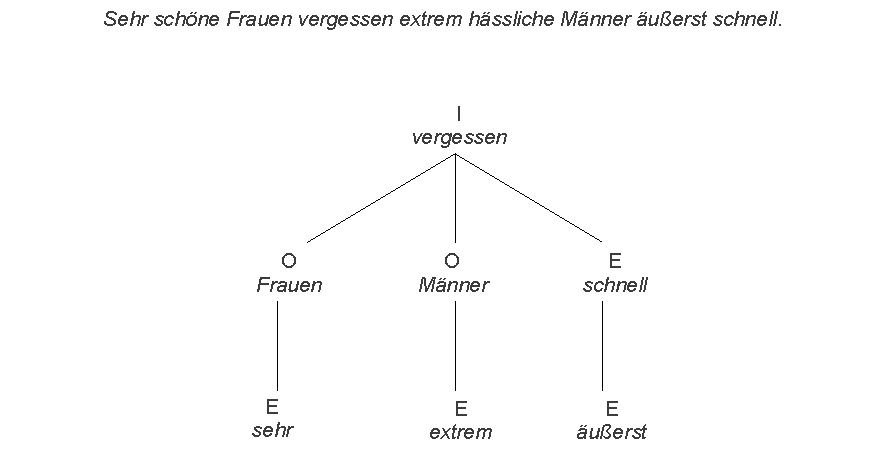
\includegraphics{images/dependenzbeziehungen_beispielsatz}
        \caption{Dependezbeziehungen zwischen Wortarten: Ein Beispiel}
        \label{fig:dependenzbeziehungen:beispielsatz}
    \end{center}
\end{figure}

Tabelle \ref{tab:dependenzbeziehungen} illustriert die besondere Bedeutung des Verbs. Es gibt allerdings auch S�tze, die ohne Verb auskommen, siehe Tabelle \ref{tab:satztypen}.

\begin{table}[htbp]
    \begin{center}
        \begin{tabular}{ l | l }
            Satztyp & Beispiel\\
            \hline
            Substantivsatz & Eine Frau f�rs Leben\\
            Adjektivsatz & Ehrlich?\\
            Adverbialsatz & Leider!\\
        \end{tabular}
        \caption{Verblose Satztypen}
        \label{tab:satztypen}
    \end{center}
\end{table}

Viele Sprachen verwenden morphologische Formen, die aus mehreren W�rtern zusammengesetzt sind, z.~B. wird Passiv, Futur oder Perfekt im Deutschen mit Hilfe von Auxiliarverben ausgedr�ckt. F�r diese F�lle gibt es in der Dependengrammatik das Konzept des mehrteiligen Nucleus \citep[Vgl.][29]{Weber1997}. Das Hilfswort wird als Auxiliar bezeichnet und dem eigentlichen Knoten, dem Auxiliat, links angef�gt, siehe Abbildung \ref{fig:mehrteiliger:nucleus}.

\begin{figure}
    \begin{center}
        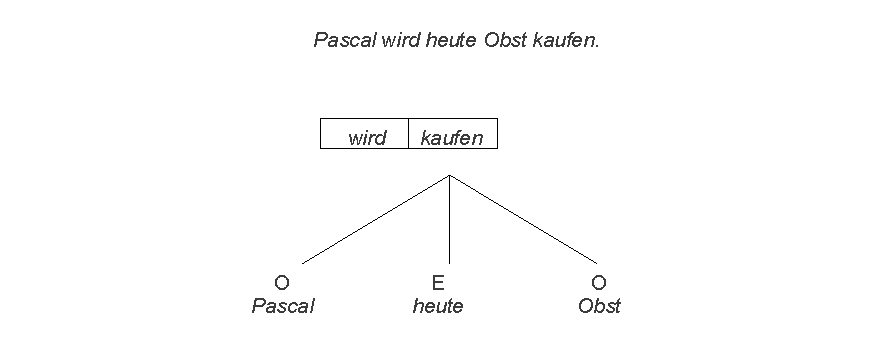
\includegraphics{images/mehrteiliger_nucleus}
        \caption{Mehrteiliger Nucleus}
        \label{fig:mehrteiliger:nucleus}
    \end{center}
\end{figure}

Anaphorische -- und ebenso kataphorische, aus struktureller Sicht besteht kein Unterschied -- Relationen werden durch eine unterbrochene Linie dargestellt \citep[Vgl.][84]{Tesniere1980}. Anaphorische Relationen k�nnen sich satz�bergreifend erstrecken, siehe Abbildung \ref{fig:anapher}.

\begin{figure}
    \begin{center}
        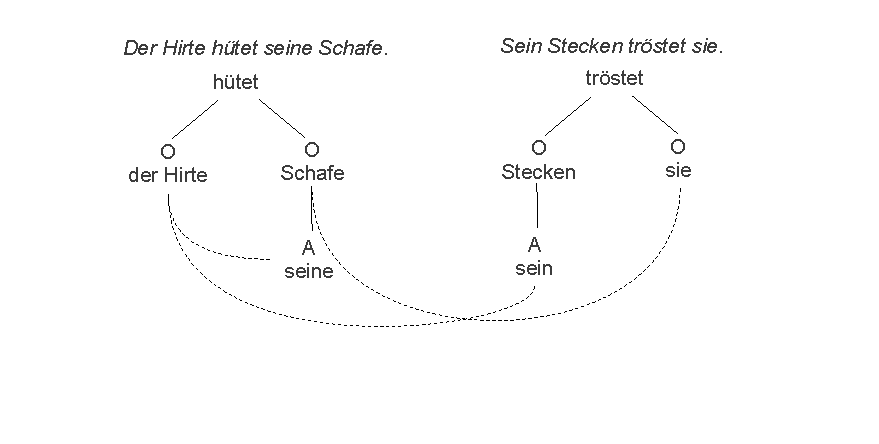
\includegraphics{images/anapher}
        \caption{Satzinterne und -�bergreifende Anaphern}
        \label{fig:anapher}
    \end{center}
\end{figure}

Anders verh�lt sich das Hilfsverb \textit{sein} in Verbindung mit pr�dikativen Adjektiven, Adverbien oder Pr�dikatsnomina. In diesen F�llen muss es als Vollverb betrachtet werden.

\subsection{Valenz}
\label{subsec:valenz}

Ein zentrals Konzept der Dependenzgrammatik ist die Valenz. Es stammt urspr�nglich aus der Chemie, wo es die F�higkeit bzw. Neigung von Atomen beschreibt, Leerstellen in der Konfiguration der �u�eren Elektronenschale bei Bildung von Verbindungen zu anderen Atomen aufzuf�llen. Analog bezeichnet Valenz in der Syntax die F�higkeit oder Neigung von W�rtern, durch andere W�rter semantsich vervollst�ndigt zu werden. So hat das Substantiv \textit{Schwester} in der Bedeutung \textit{Verwandtschaftsverh�ltnis} eine Leerstelle (\textit{wessen} Schwester?), die unbedingt gef�llt werden muss\footnote{Das Konzept der Substantivvalenz sowie der Valenz aller Wortarten ist nach Tesni�re entwickelt worden. Diese Valenz aller Wortarten wird als semantische Valenz bezeichnet und fand insbesondere in der russistischen Grammatikschreibung gro�en Anklang. Tesni�re sah eine rein syntaktische Valenz vor, die nur Verben vorbehalten war. (\citealp[Vgl.][1209]{Nuebler2003}; \citealp[Vgl. auch][89]{Helbig1995})}. Der Satz \textit{Schwester trat zur T�r hinein} ist nicht vollst�ndig, der Satz \textit{Pascals Schwester trat zur T�r hinein} hingegen schon.

In der Dependenzgrammatik spielt die Valenz des Verbs eine besonders wichtige Rolle, weil sich dadurch die Struktur des Satzes entscheidet; Tesni�re spricht ausschlie�lich von Verbvalenz \citep[Vgl.][47\,ff.]{Agel2000}, und selbst da gesteht er lediglich den Vollverben Valenzf�higkeit zu. Diejenigen Nuclei, die das Verb unbedingt braucht, um seine Leerstellen zu f�llen und somit einen grammatischen Satz zu bilden, nannte Tesni�re \textit{Aktanten}. Dabei handelt es sich um Satzelemente, die man in der traditionellen Grammatik als Subjekt und Objekt bezeichnen w�rde. Daneben sind in der Dependenzgrammatik Satzelemente vorgesehen, die zwar dem Verb unmittelbar untergeordnet sind, deren Pr�senz jedoch anders als bei den Aktanten nicht obligatorisch ist. Diese fakultativen Nuclei nannte Tesni�re \textit{Circumstanten}. �blicherweise beschreiben Circumstanten die Handlung n�her, ohne an ihr beteiligt zu sein, so wie man es vom Adverbiale kennt \citep[Vgl.][34]{Weber1997}.

Tesni�re vergleicht den Satz mit einem Theaterst�ck, dessen Handlung durch das Verb ausgedr�ckt wird. Substantive (Aktanten) sind die Akteure des St�cks und somit auf gleiche Weise allesamt der Handlung untergeordnet.
\begin{zitat}
    Die Aktanten sind Wesen oder Dinge, die auf irgendeine Art, sei es auch nur passiv, gewisserma�en als blo�e Statisten, am Geschehen teilhaben. \citep[93]{Tesniere1980}
\end{zitat}

Dem gegen�ber stehen die Umst�nde des Geschehens (Circumstanten) gleichsam als Kulisse des Theaterst�cks im Hintergrund.
\begin{zitat}
    Die Angaben bezeichnen Umst�nde der Zeit, des Ortes, der Art und Weise usw., unter denen sich das Geschehen vollzieht. \citep[93]{Tesniere1980}
\end{zitat}

Circumstanten f�llen keine Leerstellen und ihre Anzahl ist nicht begrenzt. Die Anzahl der Aktanten indes ist auf maximal drei begrenzt.

\begin{zitat}
    Wenn man die periphrastischen Formen mit tetravalenter Struktur einmal beiseite l��t, [...] scheint es, da� in keiner Sprache einfache Verbformen mit mehr als drei Valenzen vorhanden sind. \citep[179]{Tesniere1980}
\end{zitat}

Tesni�re schl�gt aber zugleich Prozeduren zur Erh�hung und Erniedrigung der Aktantenzahl vor. Um die Aktantenzahl zu erh�hen, bedarf es eines Verbs mit der Bedeutung \textit{jemanden veranlassen etwas zu tun}, z.~B. \textit{lassen}. Dieses Verfahren nennt Tesni�re Kausativierung \citep[181\,ff.]{Tesniere1980}. 

Das Verfahren zur Reduktion der Aktantenzahl nennt Tesni�re Reflexivierung \citep[193\,ff.]{Tesniere1980}. Allerdings argumentiert Weber, dass Kausativierung ebensogut durch Translation (siehe Kapitel \ref{subsec:translation}) erkl�rt werden kann. Bei Reflexivierung kann das Reflexivpronomen durchaus als Aktant angesehen werden, sofern es sich noch um das gleiche Verb handelt \citep[Vgl.][41]{Weber1997}.

In der Regel betr�gt die maximal m�gliche Anzahl der Aktanten, die ein Verb haben kann, drei. Sie werden semantisch in folgender Weise unterschieden:\\
1. Aktant: Agens (trad. Subjekt/Substantiv im Nominativ)\\
2. Aktant: Patiens (trad. direktes Objekt/Akkusativ-Objekt)\\
3. Aktant: Rezipient (trad. indrektes Objekt/Dativ-Objekt)\\
 \citep[Vgl.][100\,f]{Tesniere1980}\\
Siehe auch Tabelle \ref{tab:aktantenanzahlsaetze}.

\begin{table}[htbp]
    \begin{center}
        \begin{tabular}{ l | l }
            Beispielsatz & Anzahl der Aktanten\\
            \hline
            \rus{Svet�et.} & 0\\
            \rus{J1 gul"|j1"|j2.} & 1\\
            \rus{Pask�lp1 pokup�et j1bloki.} & 2\\
            \rus{Iv�n d�rit m�me cvet�.} & 3\\
        \end{tabular}
        \caption{Beispiels�tze mit verschieden vielen Aktanten}
        \label{tab:aktantenanzahlsaetze}
    \end{center}
\end{table}

N�bler erw�hnt die M�glichkeit regul�r vierwertiger Verben:

\begin{zitat}
    Als vierwertig bzw. quadrovalent k�nnen evtl. eingestuft werden \rus{nagraditp1} \a{belohnen (jdn. mit etw. f�r etw.)} und einige andere Verben. Diese relativ kleine Gruppe von quadrovalenten Verben wurde von Tesni�re noch nicht ber�cksichtigt.
    \citep[1207]{Nuebler2003}
\end{zitat}

In Sprachen wie den romanischen, wo etwa das Subjekt oftmals nicht als eigenst�ndiges Lexem, sondern als Verbflexiv realisiert wird, muss das Subjekt nichtsdestotrotz in der Wertigkeit entsprechend ber�cksichtigt werden. Das Ph�nomen hat gewisse �hnlichkeiten mit den elliptischen Auslassungen (siehe Kapitel \ref{subsec:auslassungen}), ist jedoch in der betreffenden Sprache als Regel und nicht als Ausnahme zu betrachten \citep[Vgl.][215\,ff]{Agel2000}.

Das Kriterium zur Unterscheidung zwischen Aktanten und Circumstanten ist formaler Natur. W�hrend Aktanten stets durch Substantive oder �quivalente wie Pronomina realisiert werden, bilden Adverbien oder deren �quivalente die Angaben \citep[Vgl.][79]{Ramers2000}.


\subsection{Auslassungen}
\label{subsec:auslassungen}

Es gibt S�tze, die formal unvollst�ndig scheinen, jedoch als v�llig akzeptabel wahrgenommen werden und im Allgemeinen auch nicht als ungrammatisch gelten. Dazu geh�ren Ellipsen z.~B. \textit{Am morgen wurde Geld gewaschen, am Abend die Gehirne.} oder Imperative \textit{Sing!}. Ebenso fehlt Passivs�tzen ohne Angabe des Agens' etwas, n�mlich dann, wenn das Agens nicht durch den Kontext bereits klar ist. Derartige Auslassungen k�nnen auf zweierlei Weisen im Stemma dargestellt werden.
\begin{enumerate}
	\item Durch Notation des fehlenden Aktanten und seiner Nummer in eckigen Klammern direkt hinter dem Verb, siehe Abbildung \ref{fig:auslassung1}.
	\item Durch Ausformulierung der fehlenden Kante, wobei das Knotensymbol in eckigen Klammern steht, siehe Abbildung \ref{fig:auslassung2}.
\end{enumerate}
In beiden Varianten wird f�r das Knotensymbol ein waagrechter Strich verwendet, wenn der Aktant nicht bekannt ist. \citep[Vgl.][36]{Weber1997}.

\begin{figure}
    \begin{center}
        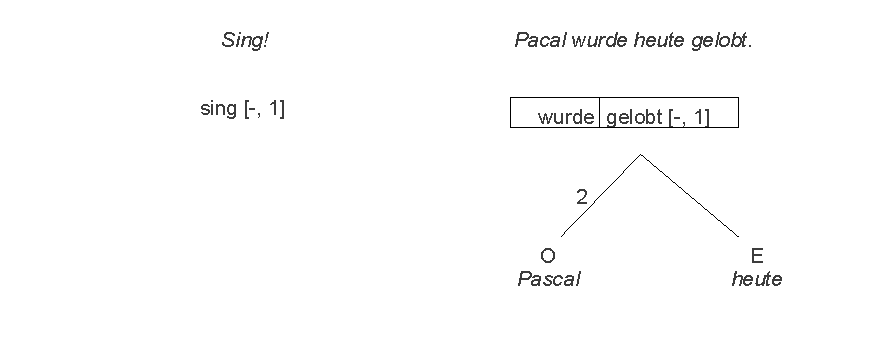
\includegraphics{images/auslassung1}
        \caption{Notation von Auslassungen mit Angabe des fehlenden Aktanten direkt beim Verb}
        \label{fig:auslassung1}
    \end{center}
\end{figure}

\begin{figure}
    \begin{center}
        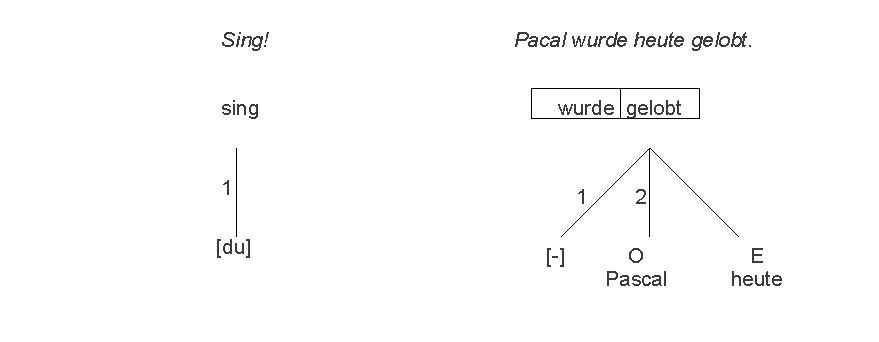
\includegraphics{images/auslassung2}
        \caption{Notation von Auslassungen mit Angabe des fehlenden Aktanten als Knoten}
        \label{fig:auslassung2}
    \end{center}
\end{figure}

\subsection{Frages�tze und Negationen}
\label{subsec:fragesaetze:negationen}

In vielen Sprachen sind invertierte Wortstellung sowie eine spezifische Intonation Merkmale von Frages�tzen. Diese Kriterien k�nnen jedoch bei der dependenzgrammatischen Darstellung der Satzstruktur nicht ber�cksichtigt werden, sodass lediglich das Fragezeichen (und evtl. Fragepartikeln) als Indikator f�r das Vorliegen eines Fragesatzes taugt. Dieses wird im Stemma demjenigen Nucleus vorangestellt, auf den sich die Frage bezieht, meist ist es das Interrogativpronomen. Tesni�re unterscheidet zwischen Nucleusfrage (Biespiel siehe Abbildung \ref{fig:nucleusfrage}) und Konnexionsfrage, (Beispiel siehe Abbildung \ref{fig:konnexionsfrage}). Im Falle der letzteren wird das Fragezeichen dem Zentralnucleus vorangestellt, das in der Regel durch ein Verb realisiert wird. \citep[Vgl.][37\,f]{Weber1997}.
In �hnlicher Weise verf�hrt man mit Negationen. F�r Negationen gilt neben dem Vorhandensein einer Negationspartikel auch die Intonation als Unterscheidungskriterium. W�hrend letzteres, wie bereits erw�hnt, bei der Strukturdarstellung ausscheidet, stellt sich beim ersteren die Frage, auf welchen Nucleus es sich bezieht. Demjenigen Nucleus, der negiert wird, stellt man die Negationspartikel voran. Beispiel siehe Abbildung \ref{fig:negation}

\begin{figure}
    \begin{center}
        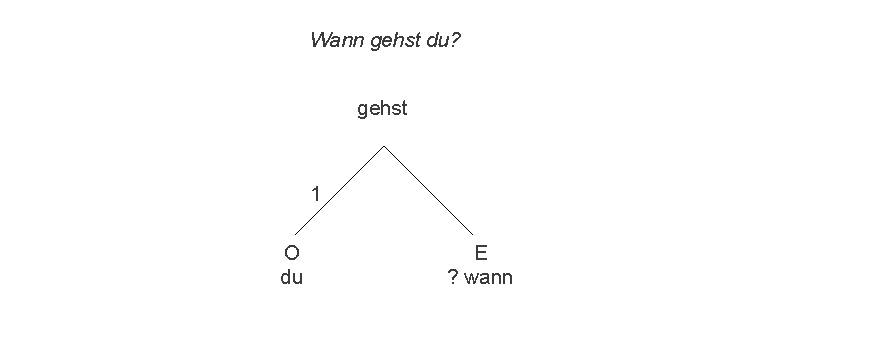
\includegraphics{images/nucleusfrage}
        \caption{Nucleusfrage}
        \label{fig:nucleusfrage}
    \end{center}
\end{figure}

\begin{figure}
    \begin{center}
        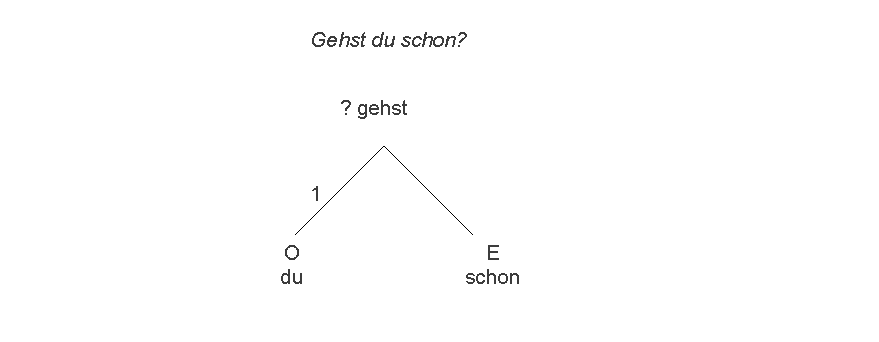
\includegraphics{images/konnexionsfrage}
        \caption{Konnexionsfrage}
        \label{fig:konnexionsfrage}
    \end{center}
\end{figure}

\begin{figure}
    \begin{center}
        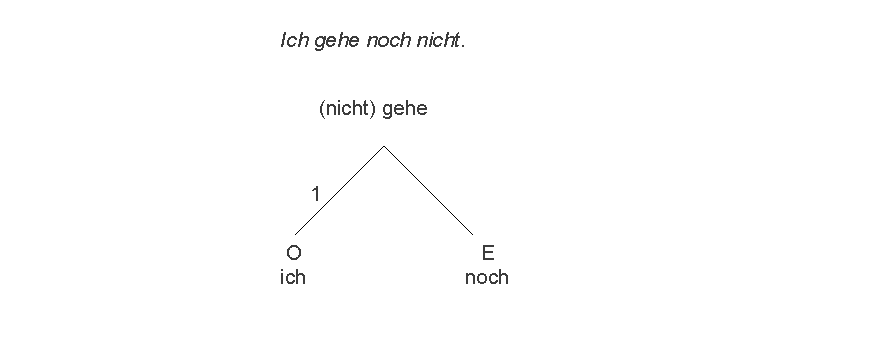
\includegraphics{images/negation}
        \caption{Negation}
        \label{fig:negation}
    \end{center}
\end{figure}

\subsection{Apposition}
\label{subsec:apposition}

Es gibt syntaktische Konstruktionen, in denen man von keiner hierarchischen Beziehung der Komponenten sprechen kann, sondern sie gleichwertig nebeneinander stellen muss. Dies ist z.~B. Der Fall im Satz \textit{Berlin, die Hauptstadt, beherbergt mehrere Universit�ten.} Sowohl das Substantiv \textit{Berlin} als auch die Nominalphrase \textit{die Hauptstadt} teilen die gleiche syntaktische Funktion und haben zugleich den selben semantischen Gehalt. Mehr noch, sie sind gegeneinander austauschbar, ohne dass sich dies in struktureller oder semantischer Hinsicht auf den Satz niederschlagen w�rde und k�nnen also nicht in eine Regens-Dependens-Beziehung gebracht werden.

Folgerichtig sieht Tesni�re f�r das Ph�nomen der Apposition deshalb eine waagerechte Konnexionslinie vor \citep[Vgl.][140]{Tesniere1980}. Beispiel siehe Abbildung \ref{fig:apposition}.

\begin{figure}
    \begin{center}
        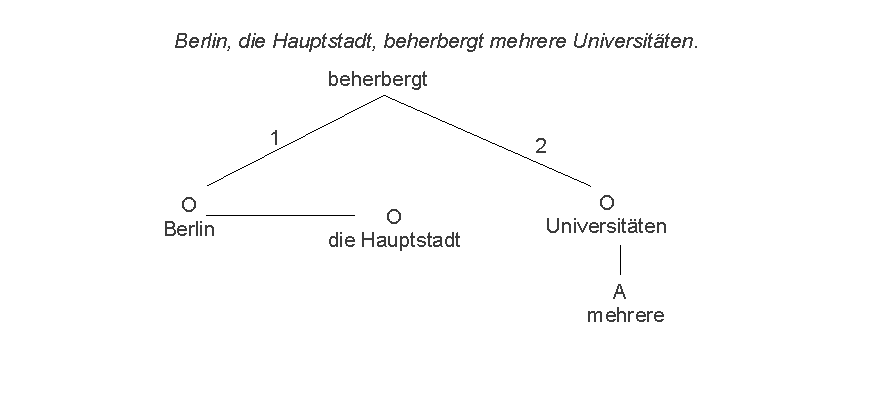
\includegraphics{images/apposition}
        \caption{Apposition}
        \label{fig:apposition}
    \end{center}
\end{figure}


\subsection{Junktion}
\label{subsec:junktion}

Bisher habe ich lediglich einfache S�tze behandelt, die aus einfachen 
Knoten bestehen. Auf das Problem der komplexen S�tze gehe ich im Kapitel 
\ref{subsec:translation} ein. Durch Junktion zusammengesetzte 
Nuclei erl�utere ich hier.

Betrachtet man einen Satz wie \textit{K�he und Ziegen grasen}, stellt sich die Frage, ob das Verb \textit{grasen} einwertig 
oder zweiwertig ist, und wenn es zweiwertig ist, ob die W�rter 
\textit{K�he} und \textit{Ziegen} beide den Status des Erstaktanten 
h�tten, und wenn nicht, welcher von ihnen der Zweit- oder gar 
Drittaktant sein sollte.

Da der Zweitaktant laut Definition die Rolle das Patiens', der 
Dritteaktant die Rolle des Rezipienten hat (siehe Kapitel 
\ref{subsec:valenz}), scheidet die zuletzt genannte Option aus. Dass mehrere 
Aktanten den selben Status, etwa den des Zweitaktanten, haben k�nnen, 
ist m�glich \citep[39\,f.]{Weber1997}. Im Falle der 
Junktion jedoch entscheidet sich Tesni�re f�r die zuerst genannte 
Variante, n�mlich die jeweils jungierten Knoten zusammenzufassen und mit dem so entstandenen B�ndel eine Verbleerstelle zu f�llen, siehe Abbildung \ref{fig:junktion1}. Allerdings sind -- bei unver�nderter Valenz des Verbs -- alle beteiligten Nuclei des B�ndels als Aktanten zu betrachten; es findet eine Vervielfachung der Aktanten statt und der Satz enthalte mehr Aktanten als zuvor.

\begin{figure}
    \begin{center}
        
\includegraphics{images/junktion1}
        \caption{Junktion zweier Erstaktanten}
        \label{fig:junktion1}
    \end{center}
\end{figure}

\begin{zitat}
    In dem Satz \textit{Alfred und Bernhard fallen} fungieren \textit{Alfred} und \textit{Bernhard} jeweils als erster Aktant. Folglich ist der erste Aktant, da durch zwei verschiedene Personen verk�rpert, hier verdoppelt.
    
    Man sollte auf keinen Fall sagen, da� dieser Satz zwei Aktanten enth�lt, kann er doch, da fallen ein monovalentes Verb ist, nur einen Aktanten haben. Aber dieser eine Aktant ist eben verdoppelt. Man mag, so man will, auch sagen, der Satz enthalte zwei erste Aktanten.
    \citep[217]{Tesniere1980}
\end{zitat}

Man kann sich die Vervielfachung der Aktanten als eine auf das Wesentliche zusammengezogene Vervielfachung ganzer S�tze vorstellen: \textit{K�he grasen} und \textit{Ziegen grasen} wird zu \textit{K�he und Ziegen grasen}.

Der Junktor, bei Tesni�re als \textit{Junktiv} bezeichnet, steht in der graphischen Darstellung zwischen den Nuclei, die er verbindet. Dar�berhinaus sind die jungierten Knoten mit einem Strich verbunden, dem Junktionsstrich. Da nur Nuclei von der selben Wortart und in der selben syntaktichen Funktion in eine Junktion treten k�nnen, ist dieser, ebenso wie im Falle der Apposition, horizontal \citep[218\,f.]{Tesniere1980}.

\subsection{Partielle Junktion}
\label{subsec:partielle:junktion}

Als ein Sonderfall der Junktion gilt die partielle Junktion, das hei�t eine Junktion zwischen regierenden, nicht aber zwischen regierten Knoten (siehe Abbildung \ref{fig:bifide}). Diese Art der Junktion hei�t \textit{bifide}, in Anlehnung an ein Ph�nomen aus der Botanik, wo solche Bl�tter als bifide bezeichnet werden, die eine tiefe Einkerbung besitzen. Da die bifiden S�tze am gemeinsamen Knoten zusammenlaufen, entsteht der Eindruck einer Einst�lpung.

\begin{figure}
    \begin{center}
        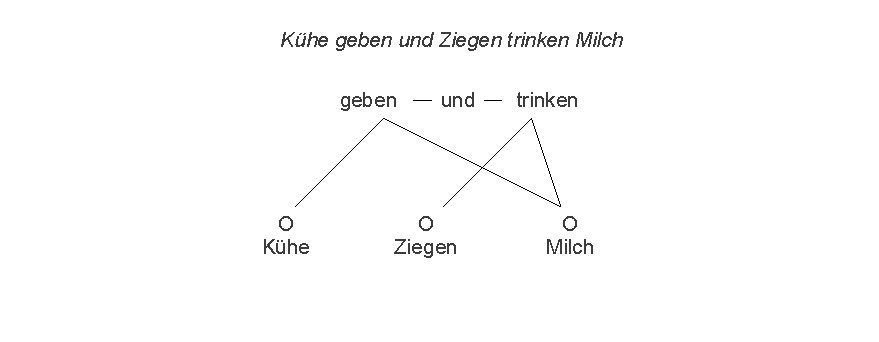
\includegraphics{images/bifide}
        \caption{Einfach bifider Satz}
        \label{fig:bifide}
    \end{center}
\end{figure}

Das Wesen der Bifidit�t liegt in der Vereinigung mehrerer S�tze, die so gestaltet ist, dass ein Nucleus mehrere S�tze bedient. Dadurch entstehen zwangsl�ufig �berschneidungen der Konnexionslinien, die umso komplexer ausfallen, je mehr Knoten in einem bifiden Satz jungiert sind.

Doppelte Bifidit�t liegt vor, wenn mehrere S�tze mit dem gleichen Zentralnucleus zusammengezogen werden.

\begin{zitat}
    Beim Stemma ergibt sich eine Schwierigkeit, weil jeder der beiden ersten Aktanten nur auf je einen der zweiten Aktanten bezogen werden darf.
    \citep[238\,f.]{Tesniere1980}
\end{zitat}

Um jener Schwierigkeit zu begegnen, bedient man sich eines horizontalen Junktionsstrichs, der im Falle einer konjunktionslosen Koordination auch keinen Junktiv anzeigt, sondern lediglich eine horizontale Linie darstellt. Die in der Abbildung \ref{fig:bifide2} dargestellten Stemmata sind �quivalent; die Notation des ausgelassenen Nucleus mit eckigen Klammern bei elliptischen Konstruktionen sollte aus Kapitel \ref{subsec:auslassungen} bekannt sein.

\begin{figure}
    \begin{center}
        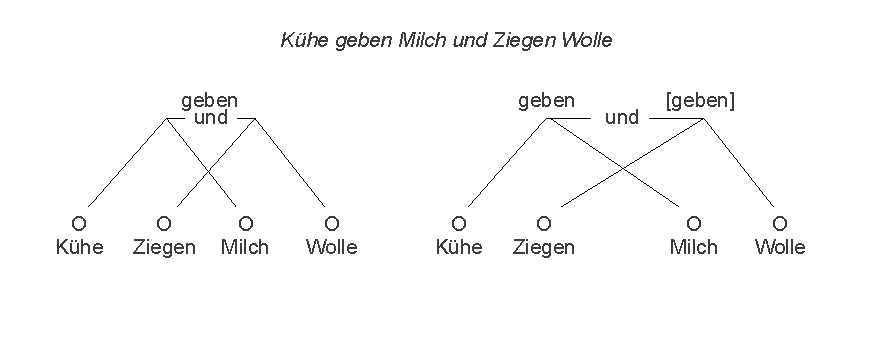
\includegraphics{images/bifide2}
        \caption{Doppelt bifider Satz}
        \label{fig:bifide2}
    \end{center}
\end{figure}

Es mag auf den ersten Blick nicht offensichtlich erscheinen, dass Vergleichss�tze ebenfalls zu den doppelt bifiden S�tzen z�hlen, siehe Abbildung \ref{fig:vergleichssatz}. \textit{Ziegen geben Milch wie K�he} kann allerdings als Zusammenziehung der S�tze \textit{Ziegen geben Milch wie K�he Milch geben} gelesen werden. \citep[Vgl.][238\,ff.]{Tesniere1980}.

\begin{figure}
    \begin{center}
        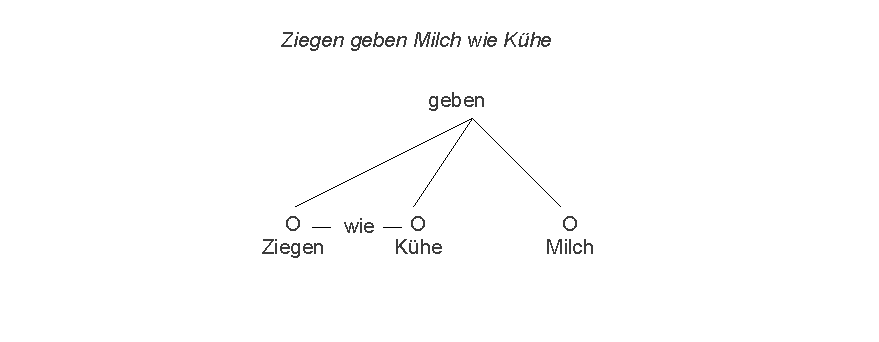
\includegraphics{images/vergleichssatz}
        \caption{Vergleichss�tze sind auch bifide}
        \label{fig:vergleichssatz}
    \end{center}
\end{figure}


\subsection{Translation}
\label{subsec:translation}

In den bisherigen Ausf�hrungen habe ich nur Haupts�tze behandelt, und die Wortklassen aller darin vorkommenden Nuclei entsprachen den aus der Schulgrammatik bekannten Wortarten. Um einen Ausdruck wie \textit{Gottes Sohn} mit den bisher vorgestellten Mitteln zu beschreiben, m�sste man ein Stemma zeichnen wie in Abbildung \ref{fig:translation1}.


\begin{figure}
    \begin{center}
        
\includegraphics{images/translation1}
        \caption{Unzul�ssige Notation}
        \label{fig:translation1}
    \end{center}
\end{figure}

Dies ist jedoch nicht zul�ssig, siehe Kapitel \ref{subsec:stemma}. Durch Konversion eines der Substantive zur Wortklasse Epitheton ergibt sich ein korrektes Stemma, siehe Abbildung \ref{fig:translation2}. Die Konversion erschent insofern sinnvoll, als im o.~g. Beispielsatz das Substantiv \a{Gottes} das Substantiv \a{Sohn} n�her beschreibt. Das Konversionsverfahren nennt Tesni�re Translation \citep[248\,ff]{Tesniere1980}.

\begin{figure}
    \begin{center}
        
\includegraphics{images/translation2}
        \caption{Zul�ssige Notation}
        \label{fig:translation2}
    \end{center}
\end{figure}

Das Novum des in der Abbildung \ref{fig:translation2} dargestellten Stemma ist das Translationssymbol, das mnemonischerweise an den Gro�buchstaben T erinnert. Die einzelnen Elemente sind:

\begin{itemize}
    \item Translationssymbol
    \item Transferend: Der Knoten vor Durchlaufen der Translation
    \item Translat: Der Knoten nach Durchlaufen der Translation
    \item Translativ: Der morphologische Markant (z.~B. Pr�position, Flexiv oder der Nullmarkant �)
\end{itemize}

Das Translat wird �ber dem Querbalken des Translationssymbols notiert. Transferend und Translativ stehen unterhalb des Querbalkens, durch den vertikalen Balken voneinander getrennt. Je nach dem, ob in der linearen Abfolge der Translativ dem Transferenden vorangeht (im Falle der Pr�positionen etwa) oder ob der Translativ auf den Transferenden folgt (im Falle der Flexive), ist das unterste St�ck des vertikalen Balkens nach links oder rechts abgeknickt. Es weist stets zum Translativ, siehe Abbildung \ref{fig:translation3}.



\begin{figure}
    \begin{center}
        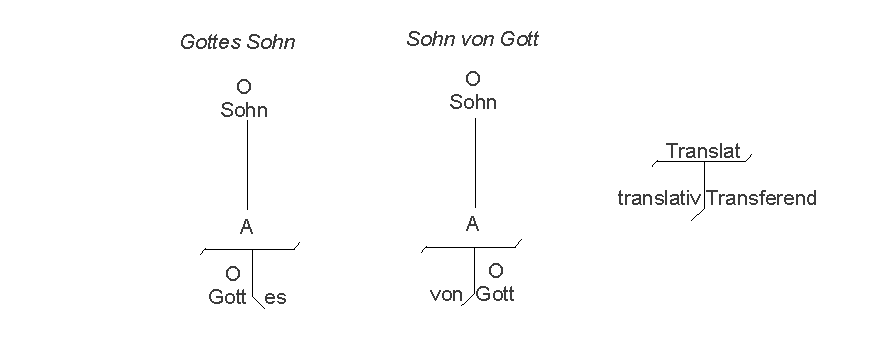
\includegraphics{images/translation3}
        \caption{Translat, Transferend und Translativ}
        \label{fig:translation3}
    \end{center}
\end{figure}


Komposita werden im Stemma in ihre Bestandteile zerlegt, und zwar auf dem Wege der Translation, oder, anders ausgedr�ckt, Translation ist der Mechanismus, der der Kompositumbildung zugrunde liegt, siehe Abbildung \ref{fig:translation4}. Dies mag in F�llen stark lexikalisierter Komposita fragw�rdig scheinen, ist jedoch grunds�tzlich sinnvoll, da dieselben Sachverhalte in Sprachen mit analytischer Formenbildung durch einzelne W�rter, mit Hilfe von Pr�positionen oder Kasusmarkierungen in Verbindung gebracht, ausgedr�ckt werden w�rden. Das Verfahren der analytischen Zerlegung qua Translation entfaltet bei der Beschreibung agglutinierender Sprachen sein volles Potential.

\begin{figure}
    \begin{center}
        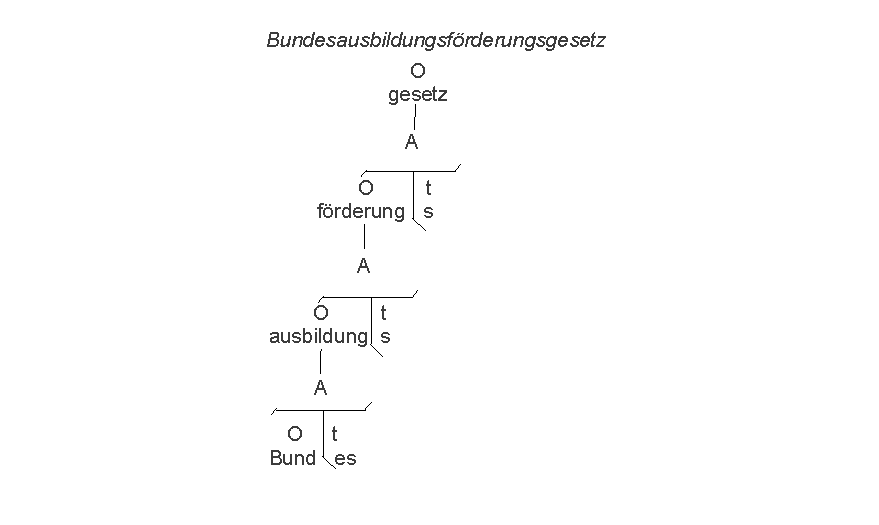
\includegraphics{images/translation4}
        \caption{Translation in Kompositum}
        \label{fig:translation4}
    \end{center}
\end{figure}

\subsection{Translation 2. Grades}
\label{subsec:translation2}

Tesni�re unterscheidet zwischen Translation 1. Grades und Translation 2. Grades. Translation 1. Grades liegt vor, wenn der Transferend kein finites Verb enth�lt, Translation 2. Grades liegt vor, wenn der Transferend selbst ein finites Verb ist oder aus einer Gruppe von W�rtern besteht, die ein finites Verb enth�lt. Translation 2. Grades dienst also dazu, Nebens�tze anzugliedern \citep[Vgl.][119]{Werner2003}. Das Translationssymbol enth�lt im Unterschied zur Translation 1. Grades einen gedoppelten Querbalken, siehe Abbildung \ref{fig:translation5}.

\begin{figure}
    \begin{center}
        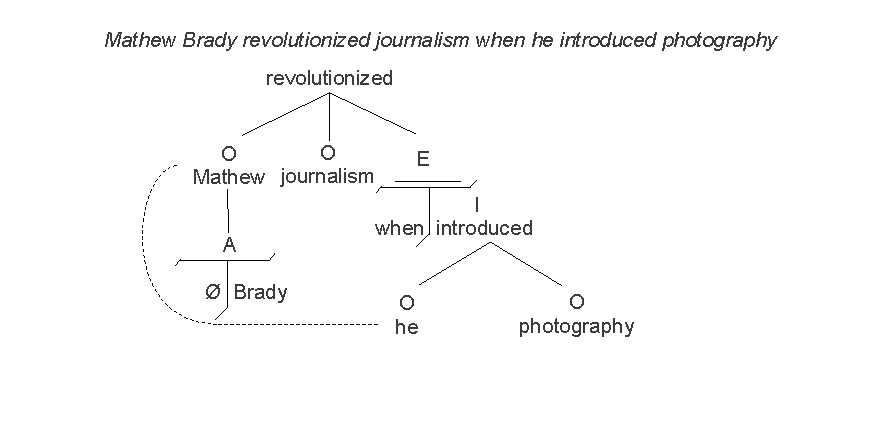
\includegraphics{images/translation5}
        \caption{Translation 2. Grades}
        \label{fig:translation5}
    \end{center}
\end{figure}

Der Nachname wird, ebenso wie Substantiv-Zus�tze von der Art \a{\textbf{C-Dur} Sonate} oder \a{Unversit�t \textbf{Trier}}, zum Epitheton translatiert \citep[Vgl.][92]{Weber1997}.

\subsection{Formale Translation}
\label{subsec:formale:translation}

Als dritter Translationstyp neben der Translation 1. Grades und der Translation 2. Grades wird die formale Translation genannt. Auf dem Wege der formalen Translation k�nnen beliebige W�rter und Wortfolgen in die Zielkategorie Substantiv (und nur in die Kategorie Substantiv) �berf�hrt werden. Da die Ausgangskategorie nicht festgelegt ist, stellt sich die Frage, ob es Translation 1. oder 2. Grades sein k�nnte, nicht; ebensowenig die Frage, ob die Translation intra- oder extranuklear abl�uft, da auch Leerw�rter als Ausgangsmaterial in Frage kommen \citep[Vgl.][276]{Tesniere1980}.

Dies k�nnen sein idiomatische Wendungen oder fremdsprachliche Zitate mit Substantivcharakter, z.~B. \textit{Sag niemals \textbf{nie}} oder \textit{Beachten Sie den \textbf{Call for Papers}}.

Alle Translationstypen k�nnen, auch kombiniert, in Mehrfachtranslationen kaskadenartig hintereinander durchlaufen werden. Zu den Kombinationsrestriktionen siehe \citep[119\,f.]{Werner2003}.

Die Translation ver�ndert die Konnexion des betroffenen Knoten nur nach oben hin. Ein O, das zum A gewandelt wurde, ist nach oben hin ein A, nach unten hin ist es ein O und kann selbst ein A regieren \citep[118]{Werner2003}.





















\clearpage
\abstand
\section{Vergleich der Dependenzgrammatik mit der Konstituentenstrukturgrammatik}
\label{sec:ksg}












\clearpage
\abstand
\section{Vergleich der Dependenzgrammatik mit der Generativen Grammatik}
\label{sec:gg}

\subsection{Theta-Rollen}
\label{subsec:theta}

Ein Modul der Generativen Grammatik, das Theta-Rollen-Modul oder $\theta$-Rollen-Modul, hat gegen�ber der Dependenzgrammatik einen deutlichen Vorteil. Durch die Theta-Rollen wird die Art und Weise, in der ...





















\clearpage
\abstand
\section{Anwendung der Dependenzgrammatik}
\label{sec:anwendung}

\subsection{Zur Vorgehensweise}
\label{subsec:vorgehensweise}

% Die insgesamt NN Stemmata 
Die Stemmata sowie der Reintext -- der ausgehend vom Stemma mitnichten rekonstruiert werden kann -- befinden sich im Anhang. Bei der Diskussion der Probleme, die mir w�hrend der Auszeichnung begegnet sind, f�hre ich den betreffenden Satz in seiner linearen Form an der jeweiligen Stelle noch einmal an. Das nicht selten sperrig ausgefallene Stemma belasse ich im Anhang, und verweise darauf unter Angabe der Seite, auf der sich die Abbildung befindet.

Bei der Benennung der einzelnen Stemmaelemente habe ich einen mittleren Grad der Ausf�hrlichkeit gew�hlt. So habe ich darauf verzichtet, in mehrteiligen Nuclei etwa Auxiliaten von Auxiliaren zu separieren oder Leerw�rter wie Partikeln zu kennzeichnen; dies ist normalerweise nicht notwenidg und Tesni�re selbst verf�hrt ebenso \citep{Tesniere1980}. Auch werden die Circumstanten nicht explizit als solche gekennzeichnet, es sollte m�glich sein, sie anhand der Wortart E zu erkennen. Translationen habe ich dergestallt illustriert, dass meist Flexionsendungen die Rolle des Translativs �bernehmen; wo es nicht sinnvoll ist, weil etwa keine Endung vorliegt, steht jeweilige grammatische Kategorie an Stelle des Translativs.

Bei der Darstellung von Partizipien habe ich die Translation (von Verben zu Adjektiv oder Adverb) nur dann herangezogen, wo es f�r den gesamten Satz von Bedeutung ist.

Auf die Darstellung satz�bergreifender Anaphern habe ich aus darstellungstechnischen Gr�nden bewusst verzichtet. Aktanten habe ich mit ihrer jeweiligen Nummer markiert. Die Wortklasse der Vollw�rter habe ich mit den jeweiligen Buchstaben ausgezeichnet; Konnexionen, Junktionen, Appositionen und Anaphern durch die jeweilige Linienart markiert, wie von Tesni�re vorgeschlagen.

\subsection{Verblose S�tze}
\label{subsec:verblose:saetze}

Die ersten interessanten Ph�nomene sind bereits im Introtext zu beobachten:
\begin{zitat}
\rus{Esli} \rus{primenit"|elp1no} \rus{k} \rus{pervomu} \rus{delu} \rus{Hodorkovskogo} \rus{i} \rus{Le}\-\rus{be}\-\rus{de}\-\rus{va} \rus{moz1no} \rus{bylo} \rus{govorit"|p1} \rus{ob} \rus{iz}\-\rus{birat"|elp1nom} \rus{primenenii} \rus{zakona,} \rus{t"|o} \rus{prigovor} \rus{Ha}\-\rus{mov}\-\rus{ni}\-\rus{qes}\-\rus{ko}\-\rus{go} \rus{suda} \rus{--} \rus{e1t"|o} \rus{uz1e} \rus{iz}\-\rus{bi}\-\rus{ra}\-\rus{t"|e}\-\rus{lp1}\-\rus{noe} \rus{primenenie} \rus{bezzakoniya}\\
(Wenn man bez�glich des ersten Verfahrens Chodorkovskis und Lebedevs von selektiver Anwendung des Gesetzes sprechen konnte, dann ist das Urteil des Gerichts in Chamovniki bereits selektive Anwendung der Gesetzeslosigkeit)\\
\citep{Nikitinskiy2010}
\end{zitat}
Die augenscheinliche Struktur offenbart sich zun�chst einmal als die eines Satzgef�ges, das aus einem Konditionalsatz besteht, dem ein Hauptsatz folgt. W�hrend der erste Teilsatz durch den Verbkomplex \rus{moz1no} \rus{bylo} \rus{govorit"|p1} (sprechen konnte) relativ leicht als Satz und durch den Subjunktor \rus{esli} (wenn) zudem in seiner Funktion identifiziert werden kann, gestaltet sich die Analyse des zweiten Teilsatzes schwieriger. Es fehlen in der langen Wortkette jegliche Verben, und die Beziehung der geh�uften Substantive untereinander offenbart sich nicht auf den ersten Blick.

�bersetzt man den Satz ins Deutsche (oder das Englische), kommt man zumindest um das obligatorische Kopulaverb \textit{sein} nicht herum; im Russischen jedoch trifft man allenthalben auf verblose S�tze, ohne dass die Grammatikalit�t darunter leiden w�rde. Im gegebenen Teilsatz liegen gleich zwei potentielle Substantivs�tze vor, wobei nur jeweils einer von ihnen zur selben Zeit Satzstatus erlangen kann -- je nach dem, ob man zum hinzuzudenkenden Verb als Adkopula \rus{prigovor} (Urteil) oder \rus{primenenie} (Anwendung) f�gt\footnote{Man k�nnte sich behelfen, indem man analog zum deutschen \textit{sein} das Verb \rus{estp1} hinzuf�gt. Wo das nicht m�glich ist, kann man es mit dem Verb \rus{yavlyatp1sya} (sein, sich erweisen als, etwas darstellen) versuchen, allerdings regiert \rus{yavlyatp1sya} den Instrumentalis, wodurch die Adkopula zum Objekt bzw. der Satzknoten zum Circumstanten w�rde.\\
\rus{Bylo} steht im ersten Teilsatz �brigens nur der Vorzeitigkeit wegen; setzte man ihn ins Pr�sens, entfiele das Verb ebenso. Es bietet sich demnach an, verblose S�tze in die Vorzeitigkeit oder Nachzeitigkeit zu setzen, und zu schauen, an welcher Stelle \rus{bylo} bzw. \rus{budet} am ehesten passt.}. Aus strukturaler Sicht ist beides m�glich, denn auf formaler Ebene liegen auf beiden Seiten des Gedankenstrichs je ein Substantiv im Nominativ samt einiger dependenter Epitheta vor. Auch die Wortstellung bietet wenig Hilfe, denn das Russische ist dank seines stark ausgepr�gten Kasussystems in dieser Hinsicht sehr frei.

Um die Frage zu beantworten, welches Substantiv den Erstaktanten und welches das Pr�dikativum realisiert, muss man semantische und pragmatische Interpretationsarbeit leisten. Hat man den pr�dikativen Teil identifiziert, k�nnte man sich verf�hrt f�hlen, einen leeren Knoten f�r die ausgelassene Kopula an die Satzspitze zu stellen. Dergleichen ist in der Dependenzgrammatik nach Tesni�re jedoch nicht vorgesehen; stattdessen soll das fehlende Verb als im Pr�dikativum inkorporiert betrachtet werden \citep[134\,f.]{Tesniere1980}; Tesni�re f�hrt an eben zitierter Stelle das Beispiel \rus{dom} \rus{nov} (das Haus ist neu) an und bezeichnet \rus{nov} (neu) als Adjektiv-Verb, wovon das Substantiv \rus{dom} (Haus) abh�ngt.

\begin{zitat}
Da aber das Regens des Substantivs normalerweise ein Verb ist, f�hrt dies zu dem Schlu�, da� das pr�dikative Adjektiv die gleiche strukturale Rolle innehat wie das Verb. Anders ausgedr�ckt: In den zitierten zyrienischen und russischen S�tzen haben die W�rter \textit{bur} \a{gut} und \rus{nov} \a{neu} dieselbe Funktion wie verbale Nexus, und die Substantive \textit{kiv} \a{Sprache} und \rus{dom} \a{Haus} sind ihre Dependentien.\\
\citep[134\,f.]{Tesniere1980}
\end{zitat}

Des Weiteren gilt es zu erkennen, welche Dependentien lediglich zur n�heren Bestimmung der Adkopula, und welche den gesamten Pr�dikatsausdruck modifizieren. Komplexe Pr�dikate m�ssen stemmatisch entwickelt werden, aber gleichzeitig als Ganzes den Aktanten und Circumstanten �bergeordnet sein. F�r die graphische Beschreibung solch schwieriger F�lle schl�gt Tesni�re das \a{entwickelte Stemma} vor, in dem das komplexe Pr�dikativum samt zugeh�riger Kopula (falls vorhanden) mit durchgezogener Linie umschlossen und somit als ein koh�rentes Ganzes dargestellt wird \citep[138\,f.]{Tesniere1980}.

Stemma zu Satz~2 siehe Abbildung \ref{fig:stemma2} auf Seite \pageref{fig:stemma2}.

\subsection{Unterscheidung zwischen Aktanten und Circumstanten}
\label{subsec:aktanten:circumstanten}

In Satz 5 
\begin{zitat}
\rus{T"|ak} \rus{qem} \rus{ot"|liqaet"|sya} \rus{sudp1ya} \rus{ot"|} \rus{ment"|a?}\\
(Und wodurch unterscheidet sich ein Richter von einem Bullen?)
\end{zitat}
{\noindent begegnet uns mit dem Verb \rus{ot"|liqatp1sya} das Problem der Dependenztheorie schlechthin, n�mlich die Unterscheidung zwischen Aktanten und Circumstanten. Nach den bisher genannten Gesichtspunkten ist \rus{sudp1ya} (Richter) Agens und damit als Erstaktant zu betrachten; \rus{qem} (wodurch) und \rus{ot} \rus{menta} (vom Bullen) sind weder Patiens noch Rezipient und k�nnen dem Rollen-Gesichtspunkt zufolge nicht Zweit- oder Drittaktant sein. Gleichwohl sind diese Syntagmen vom Verb zwingend gefordert, und zwar nicht nur in der russischen Sprache; vgl. deutsch \textit{sich unterscheiden [[von jmd./etw.] [durch etw.]]}, englisch \textit{to diverge [[from sb./sth.] [in some way]]}.}

Tesni�re war dieses Problems gewahr, fand jedoch (leider) keine L�sung.
\begin{zitat}
Dadurch kommt es zu einer empirisch nicht zu rechtfertigenden Identifikation von Form und Funktion \citep[130\,f.]{Feuillet1996}. Insbesondere hat dies zur Folge, dass Pr�positionalglieder auch dann als Zirkumstanten eingestuft werden, wenn sie obligatorisch sind bzw. eine vom Verb determinierte Pr�position enthalten [...]. So ist Tesni�re gezwungen zuzugeben, dass gewisse PPs [...] sich den Aktanten n�hern [...].
\citep[91]{Askedal2003}
\end{zitat}

Stemma zu Satz~5 siehe Abbildung \ref{fig:stemma5} auf Seite \pageref{fig:stemma5}.

\subsection{Ellipsen}
\label{subsec:ellipsen}

In Satz 3
\begin{zitat}
\rus{V} \rus{prigovore} \rus{Ha}\-\rus{mov}\-\rus{ni}\-\rus{qes}\-\rus{ko}\-\rus{go} \rus{suda,} \rus{kot"|oryi0} \rus{vesp1ma} \rus{kva}\-\rus{li}\-\rus{fi}\-\rus{ci}\-\rus{ro}\-\rus{van}\-\rus{nyi0} \rus{sudp1ya} \rus{Danilkin} \rus{poqemu-t"|o} \rus{qit"|al} \rus{t"|ak} \rus{z1e,} \rus{kak} \rus{Mut"|ko} \rus{proiznes} \rus{reqp1} \rus{na} \rus{anglii0skom,} \rus{t"|em} \rus{ne} \rus{menee,} \rus{uz1e} \rus{est"|p1} \rus{vse} \rus{i} \rus{pro} \rus{vseh.}\\
(Im Urteil des Gerichts in Chamovniki, das der �beraus qualifizierte Richter Danilkin aus irgendwelchen Gr�nden genauso verlas, wie Mutko seine Rede auf Englisch gehalten hatte, ist nichtsdestotrotz alles und �ber alle enthalten.)\\
\citep{Nikitinskiy2010}
\end{zitat}
{\noindent f�llt die Formulierung \rus{v} \rus{prigovore} ... \rus{estp1} \rus{vse} \rus{i} \rus{pro} \rus{vseh} (Im Urteil ... ist alles und �ber alle enthalten)} auf. Gemeint ist \textit{Im Urteil ist ... alles enthalten, und das alles beinhaltet alles �ber alle}. Im Stemma wir dies jedoch nicht deutlicher. Es w�re w�nschenswert, all die unter der linearen Oberfl�che liegenden Strukturen aufdecken zu k�nnen.

Stemma zu Satz~3 siehe Abbildung \ref{fig:stemma3} auf Seite \pageref{fig:stemma3}.

In Satz 7
\begin{zitat}
\rus{Nikt"|o} \rus{ne} \rus{vspom}\-\rus{nit} \rus{sle}\-\rus{do}\-\rus{va}\-\rus{t"|e}\-\rus{lya} \rus{Ka}\-\rus{ri}\-\rus{mo}\-\rus{va} \rus{i} \rus{zam} \rus{genprokurora} \rus{Biryukova,} \rus{kot"|orym} \rus{my} \rus{vse,} \rus{vklyuqaya} \rus{sudp1yu,} \rus{obyazany} \rus{ab}\-\rus{surd}\-\rus{nost"|p1yu} \rus{rexeniya,} \rus{a} \rus{vot"|} \rus{Danilkina} \rus{ne} \rus{zabudut"|.}\\
(Niemand wird sich an Ermittler Karimov und an den stellvertretenden Generalstaatsanwalt Birjukov erinnerern, denen wir alle, einschlie�lich des Richters, durch die Absurdit�t der Entscheidung verpflichtet sind, indes Danilkin wird man nicht vergessen.)\\
\citep{Nikitinskiy2010}
\end{zitat}
{\noindent ist die Ellipse \rus{nikt"|o} \rus{ne} \rus{vspomnit"|} ... \rus{a} \rus{ne} \rus{zabudut} (Niemand wird sich erinnern ... werden nicht vergessen) zu erw�hnen. Obgleich hier weder grammatische Kongruenz noch ein lexikalischer Scharnierpunkt gegeben ist, liegt gerade durch die Gegens�tzlichkeit von \rus{nikt"|o} und der nicht qua explizitem Knoten ausbuchstabierten 3.~Person Plural eine Spannung, die durch die Antonyme \rus{vspomnitp1} und \rus{zabytp1} noch verst�rkt wird. Ich habe mich entschieden, zwei S�tze daraus zu machen, und f�r das fehlende Agens im zweiten Teil das unpers�nliche \textit{man} einzusetzen.

Stemma zu Satz~7 siehe Abbildung \ref{fig:stemma7} auf Seite \pageref{fig:stemma7}.

In Satz 10
\begin{zitat}
\rus{Mne} \rus{kaz1et"|sya,} \rus{qt"|o} \rus{Danilkin} \rus{daz1e} \rus{poluqal} \rus{udovlet"|vorenie} \rus{ot"|} \rus{svo}\-\rus{ei0} \rus{sudei0skoi0} \rus{missii,} \rus{hot"|ya} \rus{iz} \rus{22} \rus{mesyacev} \rus{processa} \rus{v} \rus{t"|eqenie} \rus{dvadcat"|i} \rus{dokazyvalosp1} \rus{voobwe} \rus{ne} \rus{t"|o,} \rus{qt"|o} \rus{nado} \rus{bylo} \rus{rexit"|p1} \rus{v} \rus{per}\-\rus{vu}\-\rus{yu} \rus{oqeredp1:} \rus{t"|akova} \rus{lukavaya} \rus{t"|radiciya,} \rus{s} \rus{pomowp1yu} \rus{kot"|oroi0} \rus{rossii0skie} \rus{sudy} \rus{nauqilisp1} \rus{uhodit"|p1} \rus{ot"|} \rus{glavnyh} \rus{voprosov.}\\
(Mir scheint, dass Danilkin sogar Befriedigung durch seine richterliche Mission erfuhr, obwohl aus 22 Monaten des Prozesses im Laufe von zwanzig �berhaupt nicht das zu beweisen versucht wurde, was in erster Linie zu l�sen galt: Derart t�ckisch ist die Tradition, mit deren Hilfe die russischen Gerichte gelernt haben, von wichtigen Fragen abzuschweifen.)\\
\citep{Nikitinskiy2010}
\end{zitat}
{\noindent 
liegt mit den beiden Adverbialphrasen \rus{iz} \rus{22} \rus{mesyacev} \rus{processa} (aus 22 Monaten des Prozesses) und \rus{v} \rus{t"|eqenie} \rus{dvadcat"|i} (im Laufe von zwanzig) eine elliptische Konstruktion vor. Um die Ellipse aufzul�sen, brauchte man einen virtueller Knoten, dessen Regens \rus{te}\-\rus{qe}\-\rus{nie} und dessen Dependens \rus{dvad}\-\rus{ca}\-\rus{ti} sowie die �brige Pr�positionalphrase w�re, siehe Abbildung \ref{fig:stemma10a} auf Seite \pageref{fig:stemma10a}. Analog dazu k�nnte man auch die fehlende Kopula bei Attributivs�tzen als einen virtuellen Knoten einf�gen. Das ist von Tesni�re nicht vorgesehen, w�rde aber einiges einfacher machen. Es ist eine �berlegung wert und wird z.~B. von Pasch und Zifonun \citep[930]{Pasch2003} vorgeschlagen.
}

Diesen \a{unorthodoxen} Weg habe ich nicht beschritten, sondern w�hlte eine Variante, die nicht nur auf virtuelle Knoten verzichtet, sondern auch kompakter und besser verst�ndlich ist. 

Zuletzt l�sst sich zu diesem Satz noch anmerken, dass es sich eigentlich um zwei Haupts�tze handelt, die nicht auf dem Wege der Junktion verkn�pft sind. Das Interpunktionszeichen zwischen ihnen ist der Doppelpunkt; semantisch stellt der zweite Satz die Schlussfolgerung aus dem im ersten Satz Gesagten dar. Da jede formale Verkn�pfung fehlt, habe ich sie in zwei einzelnen Stemmata dargestellt\footnote{Es ist m�glich, die beiden S�tze zu einem zu vereinen, ohne dass sich am Inhalt etwas �ndern w�rde:\\
\rus{Mne} \rus{kaz1et"|sya,} \rus{qt"|o} \rus{t"|radiciya,} \rus{s} \rus{pomowp1yu} \rus{kot"|oroi0} \rus{rossii0skie} \rus{sudy} \rus{nauqilisp1} \rus{uhodit"|p1} \rus{ot"|} \rus{glavnyh} \rus{voprosov,} \rus{t"|akova} \rus{lukava,} \rus{qt"|o} \rus{Danilkin} \rus{daz1e} \rus{poluqal} \rus{udovlet"|vorenie} \rus{ot"|} \rus{svo}\-\rus{ei0} \rus{sudei0skoi0} \rus{missii,} \rus{hot"|ya} \rus{iz} \rus{22} \rus{mesyacev} \rus{processa} \rus{v} \rus{t"|eqenie} \rus{dvadcat"|i} \rus{dokazyvalosp1} \rus{voobwe} \rus{ne} \rus{t"|o,} \rus{qt"|o} \rus{nado} \rus{bylo} \rus{rexit"|p1} \rus{v} \rus{per}\-\rus{vu}\-\rus{yu} \rus{oqeredp1.}\\
(Mir scheint, dass die Tradition, mit deren Hilfe die russischen Gerichte gelernt haben, von wichtigen Fragen abzuschweifen, derart t�ckisch ist, dass Danilkin sogar Befriedigung durch seine richterliche Mission erfuhr, obwohl aus 22 Monaten des Prozesses im Laufe von zwanzig �berhaupt nicht das zu beweisen versucht wurde, was in erster Linie zu l�sen galt.)\\
Der Autor hatte sich wohl aus Gr�nden der aktuellen Gliederung daf�r entschieden den Konsekutivsatz auszugliedern und noch hinter das Sagzgef�ge zu positionieren.}. Der erste Teilsatz ist in Abbildung \ref{fig:stemma10} auf Seite \pageref{fig:stemma10} zu sehen, der zweite in Abbildung \ref{fig:stemma11} auf Seite \pageref{fig:stemma11}.

In Satz 38 
\begin{zitat}
\rus{Po} \rus{povodu} \rus{pervogo} \rus{prigovora} \rus{Hodorkovskomu} \rus{i} \rus{Lebedevu} \rus{mogli} \rus{byt"|p1} \rus{raznye} \rus{mneniya,} \rus{no} \rus{po} \rus{povodu} \rus{vt"|orogo} \rus{(blagodarya} \rus{absurdnoi0} \rus{formule} \rus{obvineniya)} \rus{nikakih} \rus{t"|akih} \rus{raznyh} \rus{mnenii0} \rus{uz1e} \rus{net"|.}\\
(Bez�glich des ersten Urteils �ber Chodorkivski und Lebedev k�nnte es verschiedene Meinungen geben, aber bez�glich des zweiten gibt es (dank der absurden Anklageformulierung) keine solchen verschiedenen Meinungen.)\\
\citep{Nikitinskiy2010}
\end{zitat}
{\noindent 
lie� es sich in der Phrase \rus{po} \rus{po}\-\rus{vo}\-\rus{du} \rus{vto}\-\rus{ro}\-\rus{go} (bez�glich des zweiten/Zweiten) zwar vermeiden, einen virtuellen Knoten {\lbrack}\rus{pri}\-\rus{go}\-\rus{vo}\-\rus{ra}{\rbrack} (Urteils) einzuf�gen, indem das Ordinalzahlwort \rus{vto}\-\rus{ro}\-\rus{go} (des zweiten/des Zweiten) zun�chst eine Konversioin A>O erf�hrt, um als substantiviertes Adjektiv die Bedeutung \textit{des zweiten Urteilspruchs} tragen zu k�nnen, und anschlie�end wieder O>A translatiert wird, um \rus{povod} (Anlass) in \rus{po} \rus{po}\-\rus{vo}\-\rus{du} (bez�glich/\textit{w�rtl. auf Anlass}) spezifizieren zu k�nnen. Es ist, meine ich, eine �berlegung wert, ob man an dieser Stelle nicht einen virtuellen Knoten verwenden k�nnte, wie im alternativen Stemma in Abbildung \ref{fig:stemma37a} auf Seite \pageref{fig:stemma37a} dargestellt.

Stemma zu Satz~38 siehe Abbildung \ref{fig:stemma37} auf Seite \pageref{fig:stemma37}.


\subsection{Relativpronomen als Knoten und Translator}
\label{subsec:relativpronomen}

Ebenfalls in Satz 7 gestaltet sich die Angliederung des Attributsatzes als etwas schwierig, was in der Natur des Relativpronomens liegt, zugleich Aktant und Translativ zu sein. Nun w�re es h�chst unzul�ssig, ein Wort, das in der linearen Kette nur einmal vorkommt, in der strukturalen Darstellung zweimal wiederzufinden. Um diesem Problem zu begegnen, schlagen Pasch und Zifonun \citep[930]{Pasch2003} gleich eine ganze Reihe von Herangehensweisen vor; darunter die M�glichkeit, den \a{stummen subjunktiven Anteil} (translativischen Anteil nach Tesni�re) des Pronomens als lexikalisch leeren Knoten, gleichsam als Verbindungsglied zwischen Regens und Dependens, zu installieren. Ein anderer, ebenda erw�hnter Ansatz, sieht vor, den o.g. Zwischenknoten mit dem Wort des Pronomens zu f�llen und nur dort zu platzieren; das Pronomen w�rde in einer Art Schleife sowohl das Regens des Nebensatzverbs, als auch sein Erstaktant (oder sonstiges) sein.

Tesni�re selbst \citep[349\,f.]{Tesniere1980} schlug vor, das Pronomen in seinen translativen Anteil, den er Transferem nannte, und in seinen anaphorischen Teil, den er Anaphorem nannte, aufzuteilen. Das von Tesni�re benutzte Beispielpronomen ist \textit{der}; es soll aufgespalten werden in \textit{d-} und \textit{-er}. �bertragen auf Satz 7 w�rde das Pronomen \rus{kotorym} (denen) aufgespalten werden m�ssen auf eine etymologisch zu begr�ndenden Weise (die mir nicht bekannt ist). Da dies unn�tig viel Spezialwissen erforderte und zudem die Lesbarkeit des Stemmas �ber Geb�hr beintr�chtigen w�rde, beschreite ich den alternativen Weg, f�r das Transferem die grammatische Kategorie \textit{Relativpronomen}, abgek�rzt als \textit{(Rel)}, zu verwenden. Ich st�tze mich dabei auf Weber \citep[114]{Weber1997}, der gleichsam die Vorteile der von Pasch und Zifonun \citep[930]{Pasch2003} vorgebrachten Herangehensweisen kombiniert. Das Pronomen erf�llt lediglich Knotenfunktion, wird allerdings durch eine unterbrochene Linie sowohl mit dem durch \textit{(Rel)} bezeichneten Transferem, als auch mit dem Knoten des �bergeordneten Satzes, auf das es sich anaphorisch bezieht, verbunden.

\subsection{Konnexionen zwischen Epitheta untereinander}
\label{subsec:epitheta:konnexionen}

Ebenfalls in Satz 10 
%In Satz 10 
%\begin{zitat}
%\rus{Mne} \rus{kaz1et"|sya,} \rus{qt"|o} \rus{Danilkin} \rus{daz1e} \rus{poluqal} \rus{udovlet"|vorenie} \rus{ot"|} \rus{svo}\-\rus{ei0} \rus{sudei0skoi0} \rus{missii,} \rus{hot"|ya} \rus{iz} \rus{22} \rus{mesyacev} \rus{processa} \rus{v} \rus{t"|eqenie} \rus{dvadcat"|i} \rus{dokazyvalosp1} \rus{voobwe} \rus{ne} \rus{t"|o,} \rus{qt"|o} \rus{nado} \rus{bylo} \rus{rexit"|p1} \rus{v} \rus{per}\-\rus{vu}\-\rus{yu} \rus{oqeredp1:} \rus{t"|akova} \rus{lukavaya} \rus{t"|radiciya,} \rus{s} \rus{pomowp1yu} \rus{kot"|oroi0} \rus{rossii0skie} \rus{sudy} \rus{nauqilisp1} \rus{uhodit"|p1} \rus{ot"|} \rus{glavnyh} \rus{voprosov.}\\
%(Mir scheint, dass Danilkin sogar Befriedigung durch seine richterliche Mission erfuhr, obwohl aus 22 Monaten des Prozesses im Laufe von zwanzig �berhaupt nicht das zu beweisen versucht wurde, was in erster Linie zu l�sen galt: Derart t�ckisch ist die Tradition, mit deren Hilfe die russischen Gerichte gelernt haben, von wichtigen Fragen abzuschweifen.)\\
%\citep{Nikitinskiy2010}
%\end{zitat}
{\noindent l�sst sich nicht eindeutig sagen, ob in der Phrase \rus{ot} \rus{svoei0} \rus{su}\-\rus{dei0}\-\rus{skoi0} \rus{missii} die beiden Epitheta \rus{svoei0} und \rus{su}\-\rus{dei0}\-\rus{skoi0} eigentst�ndige Knoten bilden, untereinander eine Dependenzbeziehung haben oder gar koordiniert sind. Weber bemerkt zu diesem Problem:
}
\begin{zitat}
In der Orthographie wird die Relation zwischen Attributen durch Interpunktionszeichen markiert: Komma bezeichnet \textbf{Nebenordnung} und entspricht dem \a{und}, \textbf{Unterordnung} wird durch Weglassen von Komma angezeigt [...].\\
\citep[42]{Weber1997}
\end{zitat}
Allerdings er�ffnet sich im Falle einer interpunktionslosen Aneinanderreihung die Frage, welches Epitheton das jeweils regierende ist. Ein Indiz mag sein, wie eng oder weit die Bestimmung des Substantivs durch das fragliche Adjektiv ist. Das von Weber dazu angef�hrte Beispiel ist \textit{Pascal sammelt alte englische Kupferstiche} \citep[42]{Weber1997}, wobei \textit{englische Kupferstiche} von \textit{alte} n�her bestimmt wird und somit letzteres als enger bestimmend aufzufassen w�re. Ein solches Gef�lle ist aber nicht immer gegeben; die Entscheidung liegt dann also im Ermessen des Betrachters.

Tesni�re selbst ordnet mehrere Epitheta eines Substantivs stets parallel, nicht untereinander an. Dieses Vorgehen erscheint mir intuitiv sinnvoller zu sein, denn selbst bei gegebenem Unterschied der Spezifit�t eines Eigenschaftsworts ist es eher so, dass das im jeweiligen Kontext enger fassende Epitheton die �bergeordnete Nominalphrase aus Substantiv samt dazugeh�rigen dependenten Elementen spezifizieren w�rde und nicht blo� das um eine Stufe weiter fassende Epitheton. Die von Weber vorgeschlagene Herangehensweise erscheint mir nur bei Kombinationen aus Epitheta und Adverbien sinnvoll.

Eine �hnliche Frage stellt sich zu den beiden zu Adverbien translatierten Pr�positionalphrasen \rus{iz} \rus{22} \rus{mesyacev} \rus{processa} (aus 22 Monaten des Prozesses) und \rus{v} \rus{t"|eqenie} \rus{dvadcat"|i} (im Laufe von zwanzig). In diesem konkreten Fall l�sst sich mit Hilfe des Deletionstests (siehe Kapitel \ref{subsec:konstituenten:ermittlung} auf Seite \pageref{subsec:konstituenten:ermittlung}) die letztere Phrase als unbedingt notwendig zum Verst�ndnis der ersteren identifizieren (sieht man von der Ellipse, die es erst aufzul�sen gilt, ab). In diesem Fall kann man sagen, \rus{v} \rus{t"|eqenie} \rus{dvadcat"|i} durch \rus{iz} \rus{22} \rus{mesyacev} \rus{processa} n�her bestimmt wird.

In Satz 15
\begin{zitat}
\rus{U} \rus{nego} \rus{teperp1} \rus{toz1e} \rus{estp1} \rus{kozyrp1} \rus{v} \rus{rukave,} \rus{hotya} \rus{e1to} \rus{ne} \rus{on} \rus{ego} \rus{tuda} \rus{poloz1il.}\\
(Er hat nun auch einen Ass im �rmel, obwohl nicht er selbst ihn dort hingelegt hatte.)\\
{\lbrack}\textit{w�rtl. Bei ihm ist nun auch ein Trumpf im �rmel, obwohl diesen nicht er dort hingelegt hatte.}{\rbrack}\\
\citep{Nikitinskiy2010}
\end{zitat}
{\noindent 
hat das Pr�dikativum keine Aktanten, sondern nur Circumstanten, und davon vier St�ck. Eines davon ist qua Komma abgetrennt, allerdings handelt es sich um einen Konzessivsatz und nicht um ein koordiniertes Adverbiale; aus den verbliebenen dreien stellt sich \rus{u} \rus{nego} mit Hilfe des Deletionstests als f�rs Verst�ndnis unentbehrlich heraus; \rus{te}\-\rus{perp1} und \rus{toz1e} haben keine objektiv feststellbare Pr�zedenz.
}

Stemma zu Satz~15 siehe Abbildung \ref{fig:stemma15} auf Seite \pageref{fig:stemma15}.

Es gilt also, die Beziehung von Adverbien mit gleichem Regens im Einzelfall zu pr�fen, w�hrend Epitheta mit gleichem Regens tendenziell parallel angeordnet werden sollten.

In Satz 18
\begin{zitat}
\rus{No} \rus{i} \rus{nikt"|o} \rus{iz} \rus{skolp1ko-nibudp1} \rus{obrazovannyh} \rus{i} \rus{iwuwih} \rus{qego-t"|o} \rus{lyudei0,} \rus{na} \rus{kot"|oryh} \rus{rassqit"|yvaet"|} \rus{v} \rus{svoih} \rus{planah} \rus{<modernizacii>} \rus{ne} \rus{t"|olp1ko} \rus{prezident"|} \rus{Medvedev,} \rus{ne} \rus{opredelit"|} \rus{dlya} \rus{sebya} \rus{e1t"|ot"|} \rus{prigovor} \rus{kak} \rus{spravedlivyi0.}\\
(Jedoch wird niemand von den halbwegs gebildeten und etwas suchenden Menschen, auf die nicht nur Pr�sident Medvedev in seinen Pl�nen der \a{Modernisierung} z�hlt, dieses Urteil f�r sich als gerecht empfinden.)\\
\citep{Nikitinskiy2010}
\end{zitat}
{\noindent 
ist nicht klar, ob sich \rus{skolp1ko-nibudp1} (halbwegs) nur auf \rus{obrazovannyh} (gebildet), direkt neben dem es in der linearen Kette positioniert ist, oder auch auf \rus{iwuwih} \rus{qego-t"|o} (etwas suchenden) bezieht.
}

Stemma zu Satz~18 siehe Abbildung \ref{fig:stemma18} auf Seite \pageref{fig:stemma18}.

\subsection{Sonstiges}
\label{subsec:sonstiges}

In Satz 19
\begin{zitat}
\rus{<Vor} \rus{dolz1en} \rus{sidet"|p1} \rus{v} \rus{t"|yurp1me>} -- \rus{e1t"|o} \rus{<hleba} \rus{i} \rus{zreliw>,} \rus{e1t"|o} \rus{korm} \rus{dlya} \rus{skot"|a.}\\
(\a{Der Dieb muss im Gef�ngnis sitzen} -- das ist \a{Brot und Spiele}, das ist Futter f�r das Vieh.)\\
\citep{Nikitinskiy2010}
\end{zitat}
{\noindent 
findet sich neben der in Kapitel \ref{subsec:verblose:saetze} behandelten Schwierigkeit, aufgrund des Fehlens jeglicher Verben das Subjekt und das Pr�dikat zu bestimmen, eine Besonderheit im Hinblick auf die formale Translation, der die beiden in Anf�hrungszeichen gesetzten Phrasen unterzogen werden k�nnen. W�hrend \rus{<hleba} \rus{i} \rus{zreliw>} (Brot und Spiele) als gefl�geltes Wort und festehende Wendung den Status eines Substantivs hat, ist es bei \rus{<vor} \rus{dolz1en} \rus{sidet"|p1} \rus{v} \rus{t"|yurp1me>} (der Dieb muss im Gef�ngnis sitzen) -- es handelt sich dabei um ein w�rtliches Zitat des russischen Premierministers -- auf der einen Seite als Einheit zu begreifen, auf der anderen Seite fehlt dieser �u�erung der Idiom-Charakter (siehe Kapitel \ref{subsec:formale:translation}).
}

Stemma zu Satz~19 siehe Abbildung \ref{fig:stemma19} auf Seite \pageref{fig:stemma19}.


Auch in Satz 21
\begin{zitat}
\rus{I} \rus{skolp1ko} \rus{on} \rus{dolz1en} \rus{sidet"|p1} \rus{v} \rus{t"|yurp1me} \rus{za} \rus{vseh,} \rus{esli} \rus{on} \rus{i} \rus{t"|ak} \rus{uz1e} \rus{ot"|sidel} \rus{qert"|} \rus{znaet"|} \rus{skolp1ko} \rus{i} \rus{gde} \rus{--} \rus{vsyu} \rus{z1iznp1?>.}\\
(Und wieviel soll er f�r alle im Gef�ngnis sitzen, wenn er sowieso schon wei� der Teufel wieviel und wo absa� -- das ganze Leben?)
\citep{Nikitinskiy2010}
\end{zitat}
{\noindent
kann der Phraseologismus \rus{qert} \rus{znaet} (wei� der Teufel) + Fragewort als Einheit begriffen werden. Qua formaler Translation w�rden dann einige Knoten zusammengefasst und es w�rde so ein kompakteres Stemma entstehen.
}

Stemma zu Satz21 siehe Abbildung \ref{fig:stemma12} auf Seite \pageref{fig:stemma12}.


In Satz 13
\begin{zitat}
\rus{Qt"|o} \rus{kasaet"|sya} \rus{izvest"|nogo} \rus{spora} \rus{o} \rus{nedopust"|imost"|i} \rus{<davleniya} \rus{na} \rus{sud>,} \rus{t"|o} \rus{posle} \rus{vyst"|upleniya} \rus{premp1er-minist"|ra} \rus{po} \rus{t"|elevizoru,} \rus{ya} \rus{dumayu,} \rus{k} \rus{nemu} \rus{vozvrawat"|p1sya} \rus{uz1e} \rus{ne} \rus{st"|oit"|.}\\
(Was die ber�hmte Frage �ber die Unzul�ssigkeit der \a{Druckaus�bung auf das Gericht} angeht, so denke ich, dass es nach dem Fernsehauftritt des Premier-Ministers sich nicht lohnt, zu ihr zur�ckzukehren.)\\
\citep{Nikitinskiy2010}
\end{zitat}
{\noindent
sind mehrere Stemmata m�glich. Inhaltlich �ndert sich nicht viel, wenn man \rus{ya} \rus{dumayu} (ich denke) nicht als Hauptsatz, sondern als Adverbiale in der Lesart "meiner Meinung nach" interpretiert. Auf das Stemma schl�gt sich gravierend nieder, vergleiche Abbildung \ref{fig:stemma13} auf Seite \pageref{fig:stemma13} und Abbildung \ref{fig:stemma13a} auf Seite \pageref{fig:stemma13a}.
}


In Satz 43
\begin{zitat}
\rus{I} \rus{ni} \rus{odin} \rus{qelovek} \rus{ni} \rus{s} \rus{kakimi} \rus{denp1gami,} \rus{svyazyami} \rus{ili} \rus{dolz1}\-\rus{nostp1yu} \rus{t"|ak} \rus{z1it"|p1} \rus{ne} \rus{smoz1et"|,} \rus{ne} \rus{ot"|vet"|iv} \rus{hot"|ya} \rus{by} \rus{sebe} \rus{na} \rus{vopros,} \rus{gde} \rus{vse} \rus{z1e} \rus{pravda.}\\
(Und nicht ein einziger Mensch mit allem Geld, allen Verbindungen oder Positionen wird so leben k�nnen, ohne wenigstens sich selbst die Frage beantwortet zu haben, wo denn die Wahrheit ist.)\\
\citep{Nikitinskiy2010}
\end{zitat}
{\noindent
kann das Modalverb \rus{smoz1et} (wird k�nnen) in den mehrteiligen Verbalnucleus  inkorporiert werden, siehe Kapitel \ref{subsec:stemma}. Auf der anderen Seite n�hern sich Modalverben eher den Vollverben, anders als Hilfs- oder Kopulaverben etwa, die stets einen zusammengesetzten Knoten bilden \citep[Vgl.][856]{Eichinger2003}. So lie�en sich f�r Satz 43 die beiden Stemmata konstruieren wie in Abbildung \ref{fig:stemma43} auf Seite \pageref{fig:stemma43} und Abbildung \ref{fig:stemma43a} auf Seite \pageref{fig:stemma43a}.
}










\clearpage
\abstand
\section{Fazit}
\label{sec:fazit}

Dass das Hilfsverb \textit{sein} in Kombination mit Vollverben als Auxiliar, in Kombination mit pr�dikativen Adjektiven, Adverbien oder Pr�dikatsnomina als Auxiliat auftritt (siehe Kapitel \ref{subsec:stemma}), ist problematisch.

Ebenso problematisch ist die unzureichende Abgrenzung der Kategorie und Funktion, so steht O sowohl f�r Substantiv als auch f�r Aktant; E f�r Adverb und Circumstant, \citep[Vgl.][122]{Werner2003}.

Das Aufl�sen elliptischer Konstruktionen gestaltet sich zuweilen schwierig. Genauso sind mehrdeutige S�tze, will man sie ganz genau analysieren, nur durch parallele Stemmavarianten hinreichend wiederzugeben.

Die im Russischen h�uftig zu beobachtende verblose Satzkonstruktion von der Art \rus{Ivan pekarp1} (Hans ist B�cker) ist oft nur durch semantische und pragmatische Interpretation richtig bestimmbar -- eindeutig eine kaum �berwindbare Schwierigkeit f�r maschinelle Syntaxanalyse; hier muss man sich mit statistisch-heuristischen Herangehensweisen behelfen. Das Ph�nomen der verblosen S�tze stellt die bisher gr��te H�rde f�r die Anwendung der stets vom Verb ausgehenden Dependenzgrammatik dar, ist aber, wie gezeigt wurde, von menschlichen Experten durchaus zu schaffen.

Die Beziehung von Adverbien mit gleichem Regens im Einzelfall zu pr�fen, w�hrend Epitheta mit gleichem Regens tendenziell parallel angeordnet werden sollten.

W�hrend fremdsprachliche Zitate als Einheit begriffen und zum Substantiv translatiert werden, ist es bei sonstigen Zitaten nicht klar. Es gilt also, eher mehr als weniger zu analysieren.

Stemmata eignen sich nur eingeschr�nkt, um ganze Texte zu beschreiben. Man m�sste W�nde bekritzeln, wollte man etwa ein vollst�ndiges Buch mit all den Querverweisen und Anspielungen zwischen den S�tzen angemessen wiedergeben.

Vom computerlinguistischen Standpunkt spielt die �berlegenheit der Generativen Grammatik im Hinblick auf die genauere Einordnung der Beziehungen zwischen Knoten qua Theta-Rollen, siehe Kapitel \ref{subsec:theta}, eine eher nachrangige Rolle. Denn trotz ihrer augenscheinlichen Vorteile sind die Theta-Rollen aufgrund ihrer generativ-theoretischen Natur (zumindest zum derzeitigen Stand der Forschung) kaum einsetzbar in elektronischen sprachverarbeitenden Systemen.

Der Grund f�r das fehlende Angebot kommerzieller Parsersoftware zur Verarbeitung russischer Sprache ist wohl in der au�ersprachlichen Wirklichkeit zu suchen, etwa in der mangelnden Rechtsstaatlichkeit in Russland -- denn Russland stellte das Gebiet f�r den prim�ren Absatzmarkt solcher Produkte dar. Dieser These nachzugehen ist jedoch nicht Aufgabe der Linguistik. 

















 %hier steht wohl das Meiste!
%%=================================
%%%%%%%%%%%%%%%%%%%%%%%%%%%%%%%%%%%%%%%%%%%%%%%%%%%%%%%%%%%%%%%%%%%
%% Vorlage fuer akademische Arbeiten, Gestaltungsrichtlinien der
%% Medienwissenschaft an der Universitaet Regensburg
%% 
%% Gutes Gelingen  --  Juli 2008
%% Christoph Mandl und Christoph Pfeiffer
%% http://www-mw.uni-r.de/studium/materialien 
%%
%% CC/BY-SA/3.0 - http://creativecommons.org/licenses/by-sa/3.0/
%%
%%%%%%%%%%%%%%%%%%%%%%%%%%%%%%%%%%%%%%%%%%%%%%%%%%%%%%%%%%%%%%%%

\cleardoublepage
\phantomsection
%\thispagestyle{section}
\quad\newline\quad\\
{\onehalfspacing{\listoffigures}}
%%=================================
%%%%%%%%%%%%%%%%%%%%%%%%%%%%%%%%%%%%%%%%%%%%%%%%%%%%%%%%%%%%%%%%%%%
%% Vorlage fuer akademische Arbeiten, Gestaltungsrichtlinien der
%% Medienwissenschaft an der Universitaet Regensburg
%% 
%% Gutes Gelingen  --  Juli 2008
%% Christoph Mandl und Christoph Pfeiffer
%% http://www-mw.uni-r.de/studium/materialien 
%%
%% CC/BY-SA/3.0 - http://creativecommons.org/licenses/by-sa/3.0/
%%
%%%%%%%%%%%%%%%%%%%%%%%%%%%%%%%%%%%%%%%%%%%%%%%%%%%%%%%%%%%%%%%%

\cleardoublepage
\phantomsection
%\thispagestyle{section}
\quad\newline\quad\\
{\onehalfspacing{\listoftables}}
%%=================================
%%%%%%%%%%%%%%%%%%%%%%%%%%%%%%%%%%%%%%%%%%%%%%%%%%%%%%%%%%%%%%%%%%%
%% Vorlage fuer akademische Arbeiten, Gestaltungsrichtlinien der
%% Medienwissenschaft an der Universitaet Regensburg
%% 
%% Gutes Gelingen  --  Juli 2008
%% Christoph Mandl und Christoph Pfeiffer
%% http://www-mw.uni-r.de/studium/materialien 
%%
%% CC/BY-SA/3.0 - http://creativecommons.org/licenses/by-sa/3.0/
%%
%%%%%%%%%%%%%%%%%%%%%%%%%%%%%%%%%%%%%%%%%%%%%%%%%%%%%%%%%%%%%%%%

%*********************************************************************
% changelog **********************************************************
%*********************************************************************
\cleardoublepage
\phantomsection
\newpage
\abstand
\section*{Versionen}
\label{sec:changes}
\addcontentsline{toc}{section}{Versionen}

\begin{description}
	\item Version 1.2 (8.\,Juli 2008)\\
	Kapitel 2.2: Zusammenfassung und Abstract sind nicht l�nger Bestandteil einer Abschlussarbeit.\\
	Kapitel 2.2: Abschlussarbeiten sind in digitaler Form beizuf�gen.

	\item Version 1.1 (8.\,Juni 2007)\\
	Kapitel 2.2: Anforderungen an das Titelblatt wurden ge�ndert.
\end{description} %unn�tig f�r wiss. Arbeiten
%%=================================
%%%%%%%%%%%%%%%%%%%%%%%%%%%%%%%%%%%%%%%%%%%%%%%%%%%%%%%%%%%%%%%%
%% Vorlage fuer akademische Arbeiten, Gestaltungsrichtlinien der
%% Medienwissenschaft an der Universitaet Regensburg
%% 
%% Gutes Gelingen  --  Juli 2008
%% Christoph Mandl und Christoph Pfeiffer
%% http://www-mw.uni-r.de/studium/materialien 
%%
%% CC/BY-SA/3.0 - http://creativecommons.org/licenses/by-sa/3.0/
%%
%%%%%%%%%%%%%%%%%%%%%%%%%%%%%%%%%%%%%%%%%%%%%%%%%%%%%%%%%%%%%%%%

%*********************************************************************
% Anhang *************************************************************
%*********************************************************************
\cleardoublepage
\phantomsection
\newpage
%\thispagestyle{section}
\abstand
\section*{Anhang}
\label{sec:anhang}
\addcontentsline{toc}{section}{Anhang}

%%=================================
%%%%%%%%%%%%%%%%%%%%%%%%%%%%%%%%%%%%%%%%%%%%%%%%%%%%%%%%%%%%%%%%
%% Vorlage fuer akademische Arbeiten, Gestaltungsrichtlinien der
%% Medienwissenschaft an der Universitaet Regensburg
%% 
%% Gutes Gelingen  --  Juli 2008
%% Christoph Mandl und Christoph Pfeiffer
%% http://www-mw.uni-r.de/studium/materialien 
%%
%% CC/BY-SA/3.0 - http://creativecommons.org/licenses/by-sa/3.0/
%%
%%%%%%%%%%%%%%%%%%%%%%%%%%%%%%%%%%%%%%%%%%%%%%%%%%%%%%%%%%%%%%%%

\cleardoublepage
\phantomsection
%\thispagestyle{section}
\nocite{*}
\abstand\abstand
{\footnotesize\singlespacing{{\bibliographystyle{jureco}
 \bibliography{bibtex/Literatur}}}}

%%=================================
%%%%%%%%%%%%%%%%%%%%%%%%%%%%%%%%%%%%%%%%%%%%%%%%%%%%%%%%%%%%%%%%
%% Vorlage fuer akademische Arbeiten, Gestaltungsrichtlinien der
%% Medienwissenschaft an der Universitaet Regensburg
%% 
%% Gutes Gelingen  --  Juli 2008
%% Christoph Mandl und Christoph Pfeiffer
%% http://www-mw.uni-r.de/studium/materialien 
%%
%% CC/BY-SA/3.0 - http://creativecommons.org/licenses/by-sa/3.0/
%%
%%%%%%%%%%%%%%%%%%%%%%%%%%%%%%%%%%%%%%%%%%%%%%%%%%%%%%%%%%%%%%%%

\cleardoublepage
\phantomsection
%\thispagestyle{section}

\quad\newline
\addcontentsline{toc}{section}{Eidesstattliche Erkl�rung}
\section*{Eidesstattliche Erkl�rung}

\onehalfspacing
\vspace{2cm}
\noindent Ich versichere, die vorliegende Arbeit selbstst�ndig und nur unter Benutzung der angegebenen Hilfsmittel angefertigt zu haben.
\vspace{2cm}


\begin{table*}[h]
	\centering
		\begin{tabular}{lccl}
			Gie�en, den \today & \hspace{2cm} & \dotfill & \hspace{1cm}\\
			                              & \hspace{2cm} & {\footnotesize{ \quad \quad (~Artur~~Spengler~) \quad \quad}} & \hspace{1cm}\\
		\end{tabular}
\end{table*}
 %f�r Abschlussarbeiten einkommentieren
%%=============================================================%%
\end{document}
%%=============================================================%%
